\documentclass[11pt]{article}
\usepackage[utf8]{inputenc}
\usepackage[a4paper,left=2.5cm,right=2.5cm,top=3cm,bottom=3cm]{geometry}
\usepackage{graphicx, wrapfig, caption, fancyhdr, setspace, parskip}
\usepackage[nonumberlist]{glossaries}
\usepackage[backend=biber, style=authoryear, urldate=long, url=true, doi=true, natbib=true, maxbibnames=999]{biblatex}
\usepackage{xcolor} 
\usepackage{hyperref}
\usepackage{tocloft}
\usepackage{helvet}
\usepackage{tocloft}
\usepackage{multicol}
\usepackage[ngerman]{babel}
\usepackage{microtype}
\usepackage{enumitem}
\usepackage{wasysym}
\usepackage{amssymb}
\usepackage[most]{tcolorbox}
\sloppy 

\setlength{\cftbeforesecskip}{1pt} 
\setlength{\cftbeforesubsecskip}{1pt}
\newlist{checklist}{itemize}{3}
\setlist[checklist]{label=$\square$, leftmargin=*}



\renewcommand{\familydefault}{\sfdefault}
\renewcommand{\cftloftitlefont}{\small\bfseries}
\renewcommand{\cftlottitlefont}{\small\bfseries}
\renewcommand{\headrulewidth}{0pt}
\renewcommand{\footrulewidth}{0pt}
\renewcommand{\contentsname}{Inhalt}
\onehalfspacing
\frenchspacing

\pagestyle{fancy}
\fancyhead{}
\fancyfoot[C]{} 
\fancyfoot[R]{\thepage}

\makeglossaries
\addbibresource{reference.bib}
\glstoctrue

\begin{document}

\begin{titlepage}
    \thispagestyle{empty}
    \begin{center}

        {\Huge\bfseries
        Handlungsempfehlung zu NIS2 \\EU-Richtlinie 2022/2555 \\[1.5cm]}

        \vspace{8cm}


        \noindent\rule{\textwidth}{1.2pt} \\[1cm]

        \begin{tcolorbox}[colframe=white, colback=gray!10, boxrule=0.8pt, width=0.9\textwidth, sharp corners]
            \vspace{0.5cm}
            \textbf{Autor:} \href{mailto:nikolai@furmanczak.de}{Nikolai Furmanczak} \hfill \textbf{Datum:} \today \hfill  \textbf{Version:} 1.0
            \vspace{0.5cm}
        \end{tcolorbox}

        \vfill


    \end{center}
\end{titlepage}

\pagenumbering{Roman}
\printglossaries

\tableofcontents
\newpage
\pagenumbering{arabic}
\section{Einleitung}
Dieses Dokument ist ein Leitfaden zur praxisnahen Umsetzung der EU-Richtlinie 2022/2555 (NIS2). Trotz sorgfältiger Ausarbeitung kann keine Gewähr für die Vollständigkeit der Maßnahmen übernommen werden. Zudem gelten für einzelne Sektoren spezifische Anforderungen, und jedes Unternehmen hat eigene Prozesse, sodass die Maßnahmen stets unternehmensspezifisch angepasst werden müssen. Das kann ein allgemeines Dokument nicht leisten. Es bietet aber einen ersten Orientierungsrahmen, um Planung und Umsetzung von NIS2 strukturiert anzugehen.


\subsection{Ziel der NIS2-Richtlinie}
Auf den ersten Blick mag NIS2 wie eine weitere bürokratische EU-Vorgabe wirken, die Zeit und Geld kostet. In mancher Hinsicht ist das nachvollziehbar. Dennoch enthält NIS2 viele sinnvolle Elemente für die IT-Sicherheit. Deren Grundpfeiler sind nicht primär technische Maßnahmen wie Virenscanner oder Firewalls, sondern etablierte Prozesse und organisatorische Maßnahmen, aus denen sich die Schutzmechanismen ableiten. NIS2 verfolgt daher einen ganzheitlichen Ansatz und sollte als Chance gesehen werden, die eigene IT-Sicherheitsstrategie kritisch zu hinterfragen und weiterzuentwickeln.

Ziel der EU ist es, das IT-Sicherheitsniveau von Unternehmen europaweit zu stärken. Durch die fortschreitende Digitalisierung sind IT-Systeme ein zentraler Bestandteil des wirtschaftlichen und gesellschaftlichen Lebens. Gleichzeitig nimmt die Bedrohungslage, insbesondere durch geopolitische Spannungen, stetig zu.

\subsection{Verhältnis von NIS2 zu ISO~27001, KRITIS, DORA, usw.}
Ein verbreiteter Irrtum ist, dass NIS2 zwingend ein Informationssicherheits-Managementsystem (ISMS) oder eine ISO 27001-Zertifizierung erfordert. Streng genommen verlangt NIS2 u.\,a. eine Risikoanalyse mit Sicherheitsmaßnahmen, Business Continuity, Incident Management, Supply Chain Security und IT-Awareness-Schulungen. All das ist auch ohne ISMS umsetzbar. Die Einführung eines ISMS ist dennoch empfehlenswert, falls noch keines existiert.
\newpage
Auch Unternehmen mit ISO 27001 oder vergleichbarer Zertifizierung (z.\,B. TISAX, IT-Grundschutz) müssen zusätzliche NIS2-Anforderungen erfüllen, etwa die Geschäftsleiterschulung oder die Meldung erheblicher Sicherheitsvorfälle an das BSI. Zudem gilt NIS2 immer für das gesamte Unternehmen, während bei ISO der Gültigkeitsbereich (Scope) frei gewählt werden kann. Ein Unternehmen kann außerdem mehreren Regelwerken unterliegen: Wer zusätzlich von DORA oder KRITIS betroffen ist, kann NIS2 nicht ignorieren.

\subsection{Wichtige Dokumente}
Im EU-Recht wird zwischen Richtlinien und Verordnungen unterschieden. Verordnungen gelten unmittelbar und einheitlich in allen Mitgliedstaaten. Richtlinien wie NIS2 geben nur das Ziel vor und überlassen den Mitgliedstaaten die konkrete Ausgestaltung; sie müssen daher stets in nationales Recht umgesetzt werden.

In Deutschland erfolgt dies durch das NIS2-Umsetzungsgesetz (NIS2UmsuCG), das die Anpassungen bestehender Gesetze, insbesondere des BSI-Gesetzes (BSIG), bündelt. Auch weitere Gesetze wie das Telekommunikationsgesetz werden angepasst; Unternehmen in diesen Bereichen müssen diese Änderungen ebenfalls berücksichtigen. Zentrales Referenzdokument in Deutschland ist das BSIG. Andere EU-Mitgliedstaaten haben eigene, im Detail abweichende Umsetzungsgesetze.

\begin{itemize}
    \item \href{https://eur-lex.europa.eu/legal-content/DE/TXT/PDF/?uri=CELEX:32022L2555/}{EU-Richtlinie 2022/2555}
    \item \href{https://www.bmi.bund.de/SharedDocs/gesetzgebungsverfahren/DE/Downloads/kabinettsfassung/CI1/nis2-regierungsentwurf.pdf?__blob=publicationFile&v=2}{NIS2UmsuCG}
    \item \href{https://www.gesetze-im-internet.de/bsig_2025/BJNR12D0B0025.html}{BSI-Gesetz}
\end{itemize}



\newpage

\section{Betroffenheitsprüfung}

Zunächst ist zu klären, ob die eigene Organisation überhaupt von NIS2 betroffen ist. Der Kreis der betroffenen Branchen wurde gegenüber der ersten NIS-Richtlinie deutlich erweitert. Wer bislang nicht unter NIS fiel, ist also nicht automatisch auch von NIS2 ausgenommen.

Die Anwendbarkeit hängt davon ab, ob das Unternehmen in einem der definierten Sektoren tätig ist und die Schwellenwerte für Mitarbeiterzahl und Umsatz erfüllt. Die verbindliche Auflistung der Sektoren und weitere Definitionen finden sich in Teil 8, Anlage 1 und 2 des BSI-Gesetzes. Dort wird zwischen Sektor, Branche und Einrichtungsart unterschieden; die Einrichtungsart ist am konkretesten und verweist teils auf Gesetze und Paragrafen, die eine Tätigkeit oder Einrichtung definieren.

Im Folgenden werden die relevanten Sektoren exemplarisch aufgeführt:\\
\textbf{Sektoren gemäß Anlage 1:}
\begin{itemize}
    \item Energie (z.B. Stromlieferanten, Betreiber von Übertragungsnetzen oder Erzeugungsanlagen, Energiespeicheranlagen, Fernwärmeversorger, Kraftstoff- und Heizölversorger, Gasversorger und Gasverteilernetze, Erdgasanlagen etc.)
    \item Transport und Verkehr (z.B. Luftfahrtunternehmen, Flughafenleitungsorgane, Verkehrsmanagementsysteme, Schienenverkehr, Schifffahrt, Anlagen oder Systeme für den Straßenverkehr etc.)
    \item Finanzwesen (z.B. Banken und Kreditinstitute, Finanzmarktinfrastrukturen, Handelsplätze etc.)
    \item Gesundheit (z.B. Erbringer von Gesundheitsdienstleistungen, EU-Referenzlaboratorien, Forschung und Entwicklung im Bereich Arzneimittel, Herstellung von Medizinprodukten, pharmazeutische Erzeugnisse etc.)
    \item Wasser (z.B. Trinkwasserversorgung und Abwasserbeseitigung)
    \item Digitale Infrastruktur (z.B. Internet Exchange Points, DNS-Dienstanbieter, TLD-Registries, Cloud-Computing-Dienste, Rechenzentrumsdienste, CDN, Vertrauensdienstanbieter, Betreiber öffentlicher Telekommunikationsnetze, Anbieter von Telekommunikationsdiensten, Managed Server Provider, Managed Security)
    \item Weltraum (z.B. Erbringung von weltraumgestützten Diensten, ausgenommen Kommunikationsdienste)
\end{itemize}
\newpage

\textbf{Sektoren gemäß Anlage 2:}

\begin{itemize}
    \item Transport und Verkehr, insbesondere Post- und Kurierdienste
    \item Abfallbewirtschaftung (ausgenommen Unternehmen, bei denen die Abfallbewirtschaftung nicht die Hauptwirtschaftstätigkeit darstellt)
    \item Produktion, Herstellung und Handel mit chemischen Stoffen
    \item Produktion, Verarbeitung und Vertrieb von Lebensmitteln
    \item Verarbeitendes Gewerbe und Herstellung von Waren (z.B. Medizinprodukte oder In-vitro-Diagnostika, Datenverarbeitungsgeräte, elektronische oder optische Erzeugnisse, elektrische Ausrüstungen, Maschinenbau, Kraftfahrzeuge oder -teile)
    \item Anbieter digitaler Dienste (z.B. Online-Marktplätze, Online-Suchmaschinen, soziale Netzwerke etc.)
    \item Forschungseinrichtungen
\end{itemize}
\newpage

Ist Ihr Unternehmen in einem dieser Sektoren (Anlage 1 oder 2) tätig, kann eine Betroffenheit vorliegen. Dabei ist §28 Absatz 3 BSIG zu beachten: Geschäftstätigkeiten, die im Verhältnis zur gesamten Geschäftstätigkeit vernachlässigbar sind, müssen nicht berücksichtigt werden. Das ist vor allem für Unternehmen relevant, die in mehreren Sektoren tätig sind.

Maßgeblich sind zusätzlich die Schwellenwerte: Ihr Unternehmen fällt unter NIS2, wenn \textbf{es mehr als 50 Mitarbeitende} beschäftigt \textbf{oder} wenn \textbf{Jahresumsatz und Jahresbilanzsumme mehr als 10 Mio. Euro betragen}. Mit diesem ersten Schwellenwert gilt Ihr Unternehmen als wichtige Einrichtung.

Kleine Unternehmen sind somit grundsätzlich ausgenommen, auch in betroffenen Sektoren. Eine Ausnahme bilden Monopolisten, die unabhängig von ihrer Größe erfasst werden.

Ab dem \textbf{zweiten Schwellenwert} (mehr als \textbf{250 Mitarbeitende} oder \textbf{Jahresumsatz über 50 Mio. und Jahresbilanzsumme über 43 Mio. Euro}) gilt das Unternehmen als besonders wichtig.


NIS2 unterscheidet somit zwischen wichtigen und besonders wichtigen Einrichtungen:

\textbf{Wichtige Einrichtungen:} Das Unternehmen gehört zu den Sektoren in Anlage 1 und erfüllt den ersten Schwellenwert (50 Mitarbeitende oder 10 Mio. \texteuro{} Jahresumsatz und Jahresbilanzsumme).

\textbf{Besonders wichtige Einrichtungen:} Das Unternehmen gehört zu den Sektoren in Anlage 2 oder es gehört zu Anlage 1 und erfüllt den zweiten Schwellenwert (250 Mitarbeitende oder 50 Mio. \texteuro{} Jahresumsatz und 43 Mio. \texteuro{} Jahresbilanzsumme).

Die Unterschiede betreffen vor allem Kontrolle und Registrierung: Besonders wichtige Einrichtungen können vom BSI auch ohne Anlass kontrolliert werden und müssen sich im BSI-Portal als solche registrieren. Ansonsten sind die Anforderungen identisch.

Lässt sich anhand des BSIG und der Anlagen 1 und 2 nicht eindeutig beurteilen, ob ein Unternehmen unter NIS2 fällt, ist juristische Beratung dringend anzuraten.


\newpage

\subsection{Vorbereitende Maßnahmen}

\subsection{Verantwortung der Umsetzung}

Die Gesamtverantwortung für die Einhaltung von NIS2 liegt bei der Geschäftsführung bzw. dem Management. Sie muss die Umsetzung aktiv steuern und die nötigen personellen und finanziellen Ressourcen bereitstellen.

Für die operative Umsetzung sollten geeignete Mitarbeitende (mindestens zwei, inklusive Stellvertretung) benannt werden, die koordinieren, als zentrale Ansprechpersonen dienen und die Abstimmung mit Management und Fachbereichen sicherstellen. Sie sollten künftig auch die Rolle des "IT-Sicherheitsbeauftragten" übernehmen. Regelmäßige Statustermine mit der Geschäftsführung bzw. dem Management sind empfehlenswert; Inhalte und Teilnehmende sollten kurz als Nachweis dokumentiert werden.

Fehlen Fachwissen oder interne Kapazitäten, sollten Qualifizierungsmaßnahmen durchgeführt oder, falls unumgänglich, externe Dienstleister hinzugezogen werden. Da der nachhaltige Aufbau interner Kompetenzen zentral ist, sollte Auslagerung die Ausnahme bleiben.


\subsection{Vorgaben zur Umsetzung}
NIS2 bzw. das BSIG macht keine detaillierten Vorgaben zur Umsetzung und lässt so Gestaltungsspielraum. Die Maßnahmen müssen jedoch stets angemessen sein: weder unzureichend noch unverhältnismäßig aufwendig, sondern am tatsächlichen Schutzbedarf orientiert.

Technische und organisatorische Maßnahmen sind nach dem Stand der Technik umzusetzen. Im Zweifel bieten anerkannte Standards (z.\,B. ISO 27001, BSI-200er Reihe), branchenspezifische Richtlinien oder BSI-Empfehlungen Orientierung.
\newpage
\subsection{Dokumentation}
Alle umgesetzten Maßnahmen sind nachvollziehbar und belegbar zu dokumentieren. Die Dokumentation dient als Nachweis für Umsetzung und Entscheidungen sowie der internen Steuerung und kontinuierlichen Verbesserung. Besonders wichtig ist sie bei anlassbezogenen oder stichprobenartigen Prüfungen durch das BSI oder beauftragte Dritte. Es gilt: \textbf{Ist es nicht dokumentiert, existiert es nicht.}

\subsection{PDCA-Zyklus}
NIS2 fordert u.\,a. „Kontrollen zur Bewertung der Wirksamkeit“ sowie eine „kontinuierliche Verbesserung“ der Sicherheitsmaßnahmen. Dafür sollten Prozesse zur Steuerung und Überprüfung der Umsetzung etabliert werden.

Bewährt hat sich der PDCA-Zyklus (Plan–Do–Check–Act). Er ist schlank, praxisorientiert, lässt sich nahtlos in bestehende Managementsysteme integrieren, ist auditierbar und mit Standards wie ISO 27001 kompatibel.

\subsection{Dauer und Kosten der Umsetzung}
Dauer und Kosten der Umsetzung lassen sich vorab kaum präzise beziffern. Erst eine ausführliche Gap-Analyse zeigt, wie lange die Umsetzung dauert und welche Ressourcen nötig sind.
Den größten Aufwand verursachen vermutlich Dokumentation und Prozessdefinition. Diese Aspekte werden oft vernachlässigt, selbst wenn das technische Schutzniveau relativ hoch ist.

\newpage
\subsection{Konsequenzen bei Nichterfüllung}

Das Bundesamt für Sicherheit in der Informationstechnik (BSI) ist die zentrale Aufsichtsbehörde. Art und Umfang der Kontrollen richten sich nach der Einrichtungskategorie:
\begin{itemize}
    \item \textbf{Besonders wichtige Einrichtungen:} Das BSI kann Prüfungen auch ohne konkreten Anlass anordnen
    \item \textbf{Wichtige Einrichtungen:} Kontrollen erfolgen nur bei konkretem Anlass (z.B. Sicherheitsvorfall, Hinweis, Beschwerde)
    \item \textbf{KRITIS-Betreiber:} Müssen alle drei Jahre aktiv die Umsetzung ihrer Maßnahmen nachweisen; erstmalig frühestens im Jahr 2027
\end{itemize}

Alle betroffenen Einrichtungen müssen sich innerhalb von drei Monaten nach ihrer Identifizierung beim BSI registrieren und Änderungen relevanter Angaben unverzüglich melden. Zudem sind erhebliche Sicherheitsvorfälle fristgerecht an das BSI zu melden.

Zu den potenziellen Verstößen zählen insbesondere:
\begin{itemize}
    \item Maßnahmen werden nicht korrekt, nicht vollständig oder nicht fristgerecht umgesetzt,
    \item Maßnahmen werden nicht oder nicht ordnungsgemäß dokumentiert,
    \item eine Meldung an das BSI wird nicht, nicht vollständig oder nicht rechtzeitig eingereicht,
    \item Angaben an das BSI werden nicht, nicht vollständig oder nicht fristgerecht übermittelt.
    \item Das Unternehmen verweigert oder erschwert die Zusammenarbeit mit dem BSI.
\end{itemize}

Die Bußgelder richten sich nach der Einrichtungskategorie und der Schwere des Verstoßes:
\begin{itemize}
    \item \textbf{Besonders wichtige Einrichtungen:} bis zu 10 Mio. EUR oder 2\,\% des weltweiten Jahresumsatzes, je nachdem welcher Betrag höher ist
    \item \textbf{Wichtige Einrichtungen:} bis zu 7 Mio. EUR oder 1,4\,\% des weltweiten Jahresumsatzes, je nachdem welcher Betrag höher ist
    \item \textbf{KRITIS-Betreiber bei fehlender Mängelbeseitigung:} bis zu 2 Mio. EUR
    \item \textbf{Unzureichende Nachweise:} bis zu 1 Mio. EUR
    \item \textbf{Verletzung von BSI-Anordnungen:} bis zu 500.000 EUR
\end{itemize}

\newpage
\section{NIS2 Anforderungen}

Unternehmen müssen für NIS2 die folgenden Maßnahmen nach BSIG §30 umsetzen:

\begin{itemize}
    \item Risikoanalyse und Sicherheit für Informationssysteme
    \item Konzepte und Verfahren zur Bewertung der Wirksamkeit von Risikomanagement-
    maßnahmen
    \item Bewältigung von Sicherheitsvorfällen
    \item Schwachstellenmanagement
    \item Notfall- sowie Krisenmanagement
    \item Sicherheit der Lieferkette einschließlich sicherheitsbezogener Aspekte
    \item Konzepte und Verfahren für den Einsatz von Kryptografie und gegebenenfalls Verschlüsselung
    \item Grundlegende Verfahren im Bereich der Cyberhygiene und Schulungen
    \item Sicherheitsmaßnahmen bei Erwerb, Entwicklung und Wartung von Netz-
    und Informationssystemen, einschließlich Management und Offenlegung von
    Schwachstellen
    \item Verwendung von Lösungen zur Multi-Faktor-Authentifizierung oder kontinuierlichen
    Authentifizierung, gesicherte Sprach-, Video- und Textkommunikation sowie
    gegebenenfalls gesicherte Notfallkommunikationssysteme innerhalb der Einrichtung
    \item Sicherheit des Personals, Konzepte für die Zugriffskontrolle und Management von
    Anlagen
\end{itemize}

Die Maßnahmen sollten trotz gewisser Abhängigkeiten einzeln betrachtet und umgesetzt werden. Die Reihenfolge hängt von Unternehmensgröße und bestehenden Prozessen ab; empfehlenswert ist jedoch, mit dem Risikomanagementprozess zu beginnen.

\newpage
\textbf{Checkliste: Vorbereitung}
\begin{checklist}
    \item Prüfen Sie, ob Ihr Unternehmen von NIS2 betroffen ist, durch Abgleich der Sektoren gemäß Anlage~1 und~2 des BSIG sowie der relevanten Schwellwerte.
    \item Geschäftsführung und Management über NIS2 sowie deren Verantwortlichkeiten im Rahmen von NIS2 informieren.
    \item Verantwortlichkeiten für die Analyse und Umsetzung der NIS2-Anforderungen festlegen.
    \item Eine GAP-Analyse durchführen.
    \item Entscheidung treffen, ob die Umsetzung von NIS2 intern oder mit externer Unterstützung erfolgen soll.
    \item Bei interner Umsetzung die erforderlichen personellen und finanziellen Ressourcen festlegen und freigeben.
\end{checklist}

\newpage
\subsection{IT-Asset-Management (ITAM)}
Grundlage des IT-Risikomanagements ist ein IT-Asset-Management: ein System, in dem die gesamte eingesetzte Hardware und ggf. auch Software und Lizenzen erfasst werden, beispielsweise:
\begin{itemize}
  \item Serverhardware
  \item Virtuelle Maschinen oder Container bei externen Dienstleistern
  \item Netzwerkhardware wie Switches, Router, Firewalls etc.
  \item Hardware in Büros wie WLAN-Access-Points, DHCP-Server, Drucker etc.
  \item IoT-Geräte
  \item OT-Systeme (Operational Technology)
  \item Sicherheitshardware wie Kameras, Zugangssysteme etc.
  \item Desktop-PCs, Notebooks und mobile Endgeräte wie Smartphones oder Tablets
\end{itemize}

Das Unternehmen muss definieren und dokumentieren, was ein Asset ist und ab wann es erfasst werden muss. Der Begriff kann weiter gefasst werden und Personen, Informationen oder Prozesse einschließen, etwa Geschäftsgeheimnisse, die im Risikomanagement als besonders schützenswert gelten. Grundsätzlich sollte jede betriebsrelevante Hardware erfasst werden, auch Testsysteme, da diese ebenfalls betriebskritisch sein können. Ob Server, VMs oder Container im eigenen Serverraum oder im Managed-Hosting-Rechenzentrum laufen, spielt keine Rolle. NIS2 macht keine Vorgaben zur Ausgestaltung; theoretisch genügt eine strukturierte Excel-Liste. Es gibt jedoch spezialisierte Open-Source-Lösungen wie Snipe-IT, NetBox, Ralph oder GLPI.

Neben Betriebssystem, Software und genauer Modellbezeichnung sollten, sofern verfügbar, das End-of-Life-Datum und ein verantwortlicher Asset-Owner dokumentiert werden; das hilft später u.\,a. beim Lebenszyklus- und Schwachstellenmanagement. Die Herausforderung liegt nicht nur in der initialen Erfassung, sondern im aktuellen Halten des Inventars in einer dynamischen IT-Umgebung. Je nach Infrastruktur helfen automatisierte Scanner oder Skripte, die das Netzwerk nach neuen Geräten durchsuchen, sowie Agenten, die installierte Hard- und Software erfassen und melden.
\newpage
Besonders komplex ist die Asset-Verwaltung in Cloud-Umgebungen, da Ressourcen dynamisch erstellt und gelöscht werden. Infrastructure-as-Code-Ansätze schaffen hier programmatische Sichtbarkeit; über Cloud-Provider-APIs lassen sich auch kurzlebige Ressourcen wie Container oder serverlose Funktionen erfassen.

Die Nutzung des Asset-Management-Systems muss nachvollziehbar dokumentiert sein, inklusive eines eindeutigen Prozesses für die Erfassung und die Entfernung bei Ausmusterung. Ein Prozessverantwortlicher sollte die Einhaltung kontrollieren, den Prozess verbessern und als zentraler Ansprechpartner dienen.

Für Datenträger und Geräte mit sensiblen Informationen muss ein Prozess zur sicheren Löschung bzw. Entsorgung definiert werden, idealerweise als verbindliche, im Unternehmen kommunizierte Arbeitsanweisung.

Eine weitere Herausforderung ist Schatten-IT: Geräte oder Software, die ohne Genehmigung und Wissen der IT-Abteilung genutzt und daher nicht überwacht und verwaltet werden. Neben einer Richtlinie zur Nutzung privater Hardware (BYOD, Bring Your Own Device) sollte die IT weitere Maßnahmen ergreifen, etwa automatische Netzwerkscans nach unbekannten Geräten bzw. MAC-Adressen.
\newpage
\textbf{Checkliste: Asset-Management}
\begin{checklist}
  \item Festlegen, was in der Organisation als Asset gilt (z.\,B. IT-Systeme, Software, Daten, Services)
  \item Definieren, welche Informationen zu einem Asset erfasst werden müssen (z.\,B. Name, Standort, Owner, Zweck, Hardware-Typ, Betriebssystem, Schnittstellen)
  \item Festlegen eines fachlichen Asset Owners mit klarer Verantwortung
  \item Klassifizieren der Assets nach Kritikalität und Schutzbedarf (Verfügbarkeit, Integrität, Vertraulichkeit)
  \item Auswahl eines geeigneten Tools zur zentralen Erfassung und Pflege der Assets
  \item Definieren eines Prozesses zur Identifikation und initialen Erfassung neuer Assets
  \item Definieren eines Prozesses zur Pflege und Aktualisierung von Asset-Informationen bei Änderungen
  \item Definieren eines Prozesses zur Außerbetriebnahme und Entsorgung von Assets
  \item Definieren eines Prozesses zur sicheren Vernichtung von Datenträgern oder Geräten mit sensiblen Informationen
  \item Regelmäßiger Abgleich zwischen dokumentiertem Asset-Bestand und tatsächlicher Umgebung (Dokumentation vs. Realität)
\end{checklist}
\newpage
\subsection{IT-Risikomanagement}
Das IT-Risikomanagement ist ein zentraler Punkt von NIS2. Ziel ist es, die Infrastruktur hinsichtlich potenzieller Risiken zu bewerten und diesen mit technischen oder organisatorischen Maßnahmen zu begegnen. Ergebnis ist also nicht nur die Risikoanalyse selbst, sondern auch die daraus abgeleiteten Maßnahmen.

Zunächst muss die Organisation den Begriff Risiko für sich definieren. Typischerweise sind Risiken Ereignisse, die bei Eintritt die Informationssicherheitsziele (Vertraulichkeit, Verfügbarkeit, Integrität) oder Geschäftsziele beeinträchtigen. Vor der Risikoanalyse sollten zudem folgende Begriffe bestimmt werden:

Das \textbf{Gesamtrisikoprofil} fasst alle relevanten Risiken der Organisation verdichtet zusammen und beantwortet die Frage: Wie riskant ist unser Unternehmen insgesamt? Neben IT-Risiken fließen operationelle, finanzielle und strategische Risiken ein. Ein vollständiges Bild entsteht erst mit ESG-Risiken (Environmental, Social, Governance), die zunehmend regulatorische Bedeutung gewinnen.

\textbf{Risikotoleranz} beschreibt, wie viel Risiko eine Organisation bewusst eingehen will, um ihre strategischen Ziele zu erreichen.

\textbf{Inhärentes Risiko} und \textbf{Residualrisiko}: Das inhärente Risiko (Bruttorisiko) ist das Risiko vor jeglichen Gegenmaßnahmen, das Residualrisiko (Restrisiko) das nach Umsetzung aller Maßnahmen verbleibende Risiko. Ihre Differenz zeigt, wie wirksam die Kontrollen sind. Geschäftsleitungen müssen verstehen, dass Risiken nie auf null sinken und sie das Restrisiko formal akzeptieren müssen.

Das \textbf{Risikodeckungspotenzial} beschreibt, wie viel Risiko eine Organisation finanziell und organisatorisch abfedern kann, ohne in existenzielle Schwierigkeiten zu geraten, typischerweise durch Eigenkapital, liquide Reserven und Versicherungen. Die \textbf{Risikotragfähigkeit} setzt das Gesamtrisikoprofil ins Verhältnis zum Deckungspotenzial: Liegt unser Gesamtrisiko innerhalb dessen, was wir verkraften können? Wenn nicht, besteht akuter Handlungsbedarf.
\newpage
Zusätzlich empfiehlt es sich, Risikoklassen anhand des Risikodeckungspotenzials zu definieren. Die niedrigste Klasse umfasst Risiken mit vernachlässigbaren Auswirkungen. Ein Beispiel:

\tcbset{colback=gray!5!white, colframe=gray!70!black, boxrule=0.3mm, arc=1mm, left=1mm, right=1mm, top=0.5mm, bottom=0.5mm}

\begin{tcolorbox}[title=Klasse 1: Minimal]
Kaum Auswirkungen, Verluste unter 1.000\texteuro. Risiko akzeptabel, keine Maßnahmen.
\end{tcolorbox}

\begin{tcolorbox}[title=Klasse 2: Niedrig]
Geringfügige Beeinträchtigungen, Verluste 1.000–10.000\texteuro. Überwachung empfohlen.
\end{tcolorbox}

\begin{tcolorbox}[title=Klasse 3: Mittel]
Spürbare Auswirkungen, Verluste 10.000–100.000\texteuro. Maßnahmen erforderlich.
\end{tcolorbox}

\begin{tcolorbox}[title=Klasse 4: Hoch]
Erhebliche Störung, Verluste 100.000–1.000.000\texteuro. Sofortiges Eingreifen notwendig.
\end{tcolorbox}

\begin{tcolorbox}[title=Klasse 5: Kritisch]
Existenzbedrohend, Verluste $>\,$1.000.000\texteuro. Notfallmaßnahmen zwingend.
\end{tcolorbox}

Klassen, Definitionen und Werte dienen nur als Orientierung und können je nach Organisation angepasst werden.

Als Nächstes ist ein IT-Risikomanagement-Modell auszuwählen und die Entscheidung begründet zu dokumentieren. Verbreitete Frameworks sind ISO 27005, NIST RMF, COSO ERM und BSI 200-3. Sie haben alle ihre Berechtigung, sind aber komplex und für kleinere Unternehmen möglicherweise zu umfangreich. NIS2 verlangt nur angemessene Maßnahmen. Ist das Unternehmen zu klein, fehlen personelle Kapazitäten oder sind die Prozesse der Frameworks zu starr, ist ein eigenes Risikomanagement legitim. Auch dies ist in der Dokumentation zu begründen. Wichtig ist, dass der Prozess für alle IT-Systeme identisch abläuft. Er darf (und muss ggf.) punktuell angepasst werden, aber nicht ohne Grund, da sonst Vergleichbarkeit und Kontinuität leiden. Jedes IT-Risikomanagement umfasst mindestens vier Phasen: Risiken identifizieren, Risiken bewerten, Risiken behandeln und Monitoring.

Der Prozess muss regelmäßig wiederholt werden, um zu prüfen, ob Maßnahmen noch aktuell sind oder neue Risiken entstanden sind, und sollte kontinuierlich verbessert werden. Ebenso ist er durchzuführen, wenn Komponenten hinzugefügt oder ausgetauscht werden.
\newpage
\subsubsection{Phase 1: Risiken identifizieren}
In der ersten Phase sollen potenzielle Risiken möglichst vollständig identifiziert werden, unabhängig von Eintrittswahrscheinlichkeit oder Schwere. Ziel ist nicht die Bewertung oder Priorisierung, sondern alle relevanten Risikoszenarien sichtbar zu machen.

Im Fokus stehen Risiken für Verfügbarkeit, Integrität und Vertraulichkeit von Informationen, IT-Systemen und unterstützenden Prozessen. Ausgangspunkt ist in der Regel das IT-Asset-Management: Für jedes Asset wird betrachtet, welchen Bedrohungen und Schwachstellen es ausgesetzt sein könnte. Ähnliche Systeme können zusammengefasst werden. So besteht bei nahezu jeder Hardware das Risiko eines Ausfalls von Festplatten, Netzteilen oder anderen Komponenten. Auch Systeme gleicher Funktion, etwa Datenbank- oder Webserver, lassen sich gruppieren, um die Übersicht zu wahren.

Die Identifikation sollte strukturiert, aber bewusst offen gestaltet werden. Bewährt hat sich ein gemeinsames Brainstorming mehrerer Mitarbeitender mit Kenntnis der IT-Umgebung und Geschäftsprozesse. Alternativ sammeln zunächst kleine Gruppen eigene Risikoszenarien, die anschließend zusammengeführt, diskutiert und ergänzt werden. Methoden wie Brainwriting oder die 6-3-5-Methode helfen, auch weniger offensichtliche Risiken sichtbar zu machen.

Neben technischen sind auch organisatorische, personelle und externe Risiken zu berücksichtigen, etwa Abhängigkeiten von Dienstleistern, Ausfall von Schlüsselpersonal oder eine veränderte Bedrohungslage. Wer wenig Erfahrung hat, kann sich an Rahmenwerken orientieren, etwa am BSI-Standard 200-3, der ein schlankes Risikomanagement-Framework sowie eine Liste von Gefährdungskategorien bereitstellt.
\newpage
\subsubsection{Phase 2: Risiken bewerten}
Anschließend werden die Risiken bewertet, um Relevanz und Priorität einzuschätzen. Die wichtigsten Kriterien sind \textbf{Eintrittswahrscheinlichkeit} und \textbf{Schadauswirkung}. Denkbar sind weitere Faktoren wie Erkennbarkeit, Kontrollierbarkeit, Kaskadeneffekte, Wiederherstellungszeit oder die Zeit bis zum Schadenseintritt.

Für ein praktikables Risikomanagement genügt es zunächst, sich auf Eintrittswahrscheinlichkeit und Schadauswirkung zu konzentrieren. Weitere Faktoren können bei besonders kritischen oder komplexen Risiken ergänzt werden.

Bewertet wird üblicherweise auf einer numerischen Skala (z.\,B. 1 bis 5), deren Werte klar beschrieben sein müssen, um eine einheitliche Bewertung zu ermöglichen. Die Bewertung ist kein rein technischer Vorgang, sondern ein Abstimmungsprozess mit verschiedenen Personen und Fachbereichen, sodass unterschiedliche Perspektiven einfließen.

Objektive Messwerte gibt es selten; Einschätzungen beruhen oft auf Erfahrung, Annahmen und fachlichem Urteil. Um diese Subjektivität zu reduzieren, sollten Risiken gemeinsam diskutiert und Bewertungen nachvollziehbar begründet werden, mit dem Ziel einer konsistenten Einschätzung.

Aus beiden Faktoren ergibt sich der Risikowert: $Schadauswirkung \times Eintrittswahrscheinlichkeit$. Er dient als vereinfachte Kennzahl zur Priorisierung: Je höher der Wert, desto kritischer das Risiko und desto dringlicher die Behandlung.
\newpage
\begin{figure}[htbp]
  \centering
  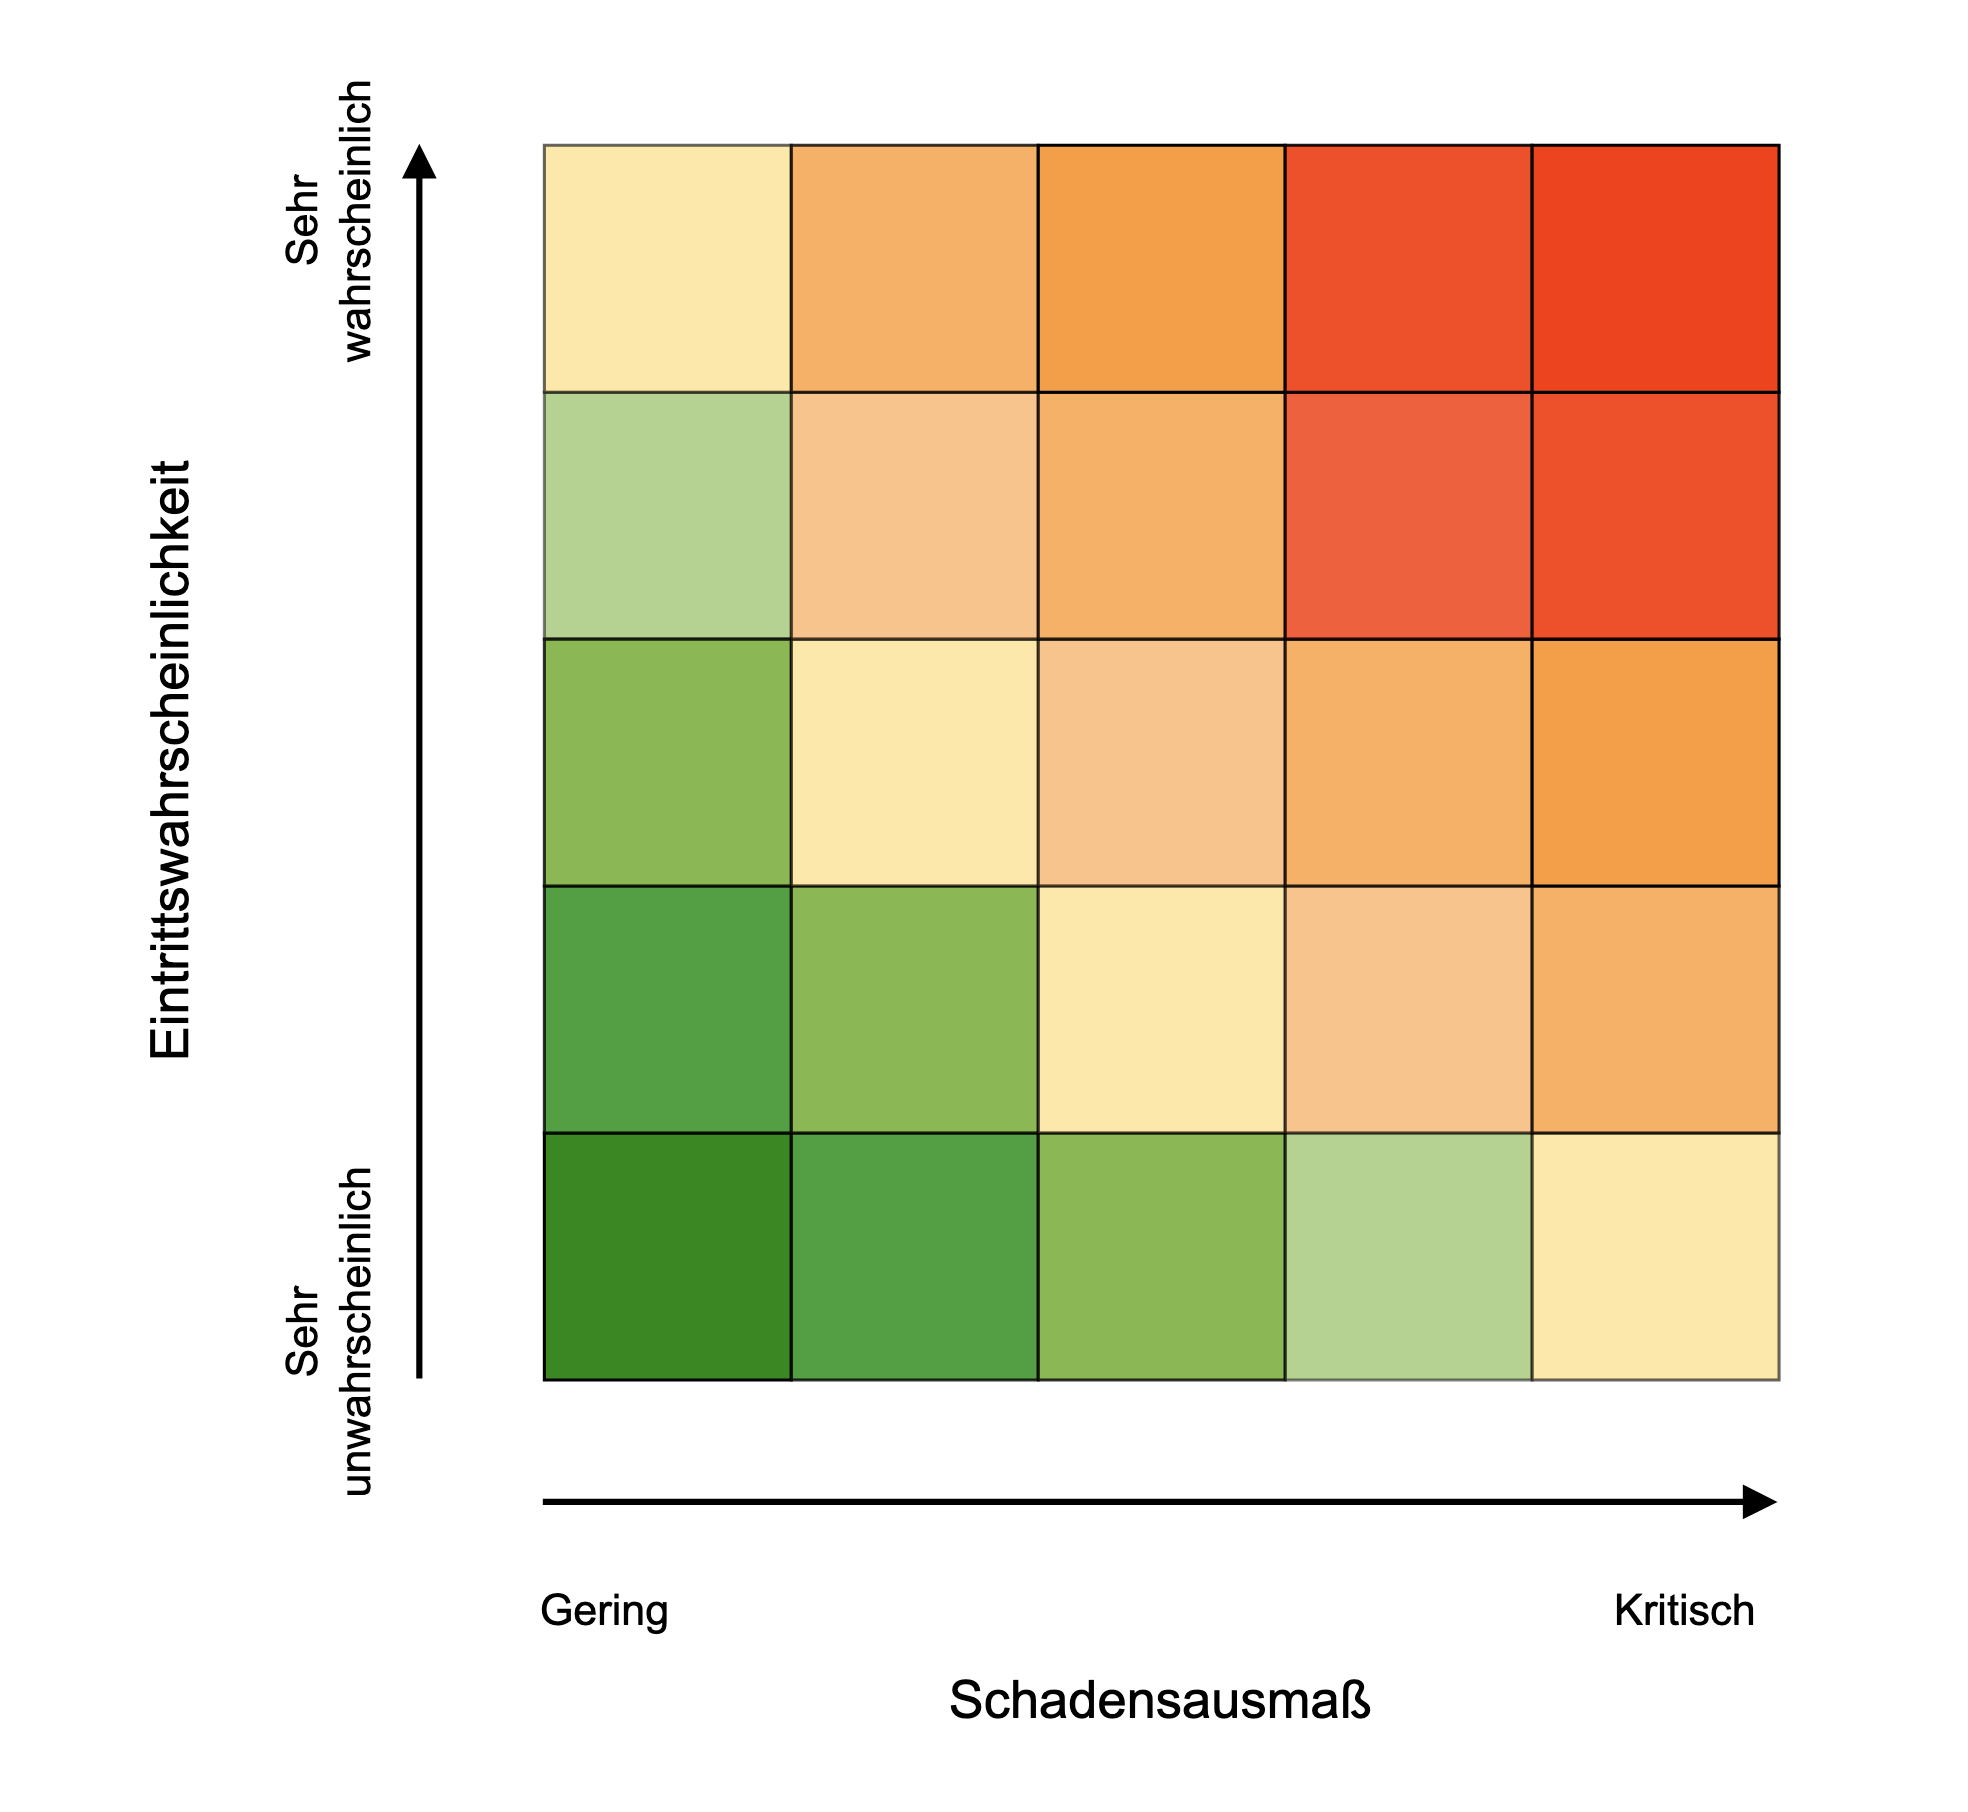
\includegraphics[width=0.55\textwidth]{images/Risikomatrix.png}
  \caption{Beispiel einer Risikomatrix}
  \label{fig:risikomatrix}
\end{figure}

Zur Übersicht können die bewerteten Risiken in einer Risikomatrix mit Schadauswirkung und Eintrittswahrscheinlichkeit als Achsen dargestellt werden, sodass kritische Risiken auf einen Blick erkennbar sind.



\newpage
\subsubsection{Phase 3: Maßnahmen ergreifen}

Risiken werden nach Priorität behandelt, hoch bewertete zuerst. Grundsätzlich gibt es vier Behandlungsoptionen:
\begin{itemize}
  \item \textbf{Vermeiden}: Das Risiko wird vermieden, indem die zugrunde liegende Tätigkeit nicht durchgeführt oder ein IT-System nicht betrieben bzw. abgeschaltet wird.
  \item \textbf{Mindern}: Durch technische oder organisatorische Maßnahmen wird die Eintrittswahrscheinlichkeit oder die Schadauswirkung eines Risikos reduziert.
  \item \textbf{Transferieren}: Das Risiko wird ganz oder teilweise an Dritte übertragen, beispielsweise durch Outsourcing oder den Abschluss von Versicherungen.
  \item \textbf{Akzeptieren}: Das Risiko wird bewusst akzeptiert, da es als tragbar eingeschätzt wird.
\end{itemize}

Die Wahl hängt von den Gegebenheiten der Organisation ab. In der Praxis werden Risiken meist gemindert, etwa durch Zwei-Faktor-Authentifizierung gegen die unbefugte Übernahme von Benutzerkonten. Welche Maßnahmen geeignet sind, hängt u.\,a. von Kosten, Nutzen und Umsetzungsaufwand ab. Fachabteilungen oder IT-Teams können Maßnahmen vorschlagen; über Priorisierung und Ressourceneinsatz entscheidet in der Regel das Management.

Beim Transfer durch Outsourcing oder Versicherungen verschwindet das Risiko nicht: Es entstehen neue Abhängigkeiten, und die Verantwortung für Auswahl, Steuerung und Überwachung der Dienstleister bleibt bestehen.

Das Vermeiden durch Unterlassen einer Aktivität oder Abschalten eines Systems kommt vor allem bei neuen Vorhaben oder nicht geschäftskritischen Systemen in Betracht, da es bei bestehenden Infrastrukturen oft nur eingeschränkt möglich ist.

Akzeptiert werden vor allem Risiken mit geringer Auswirkung oder solche, die als tragbar gelten. Akzeptieren heißt nicht ignorieren: Die Organisation kennt durch die Analyse Eintrittswahrscheinlichkeit und möglichen Schaden und entscheidet sich bewusst gegen weitere Maßnahmen.

Unabhängig von der Strategie verbleibt meist ein Restrisiko. Behandlungsentscheidung und akzeptiertes Restrisiko sind mit kurzer Begründung zu dokumentieren; das erhöht die Nachvollziehbarkeit bei Audits und erneuten Risikoanalysen.
\newpage
Manche Risiken sollten im Business Continuity Management (BCM) behandelt werden: solche, die kritische Geschäftsprozesse bedrohen (ob technisch oder organisatorisch) und deren Unterbrechungseffekte definierte Toleranzen überschreiten, insbesondere wenn ihre Auswirkungen das Risikodeckungspotenzial bzw. die Risikotragfähigkeit übersteigen. Sie lassen sich nicht allein durch Prävention oder Kontrollen beherrschen, sondern erfordern vorbereitete Maßnahmen zur Aufrechterhaltung des Geschäftsbetriebs und zum Wiederanlauf. Während das IT-Risikomanagement Eintrittswahrscheinlichkeit und Schadenshöhe reduziert, sichert das BCM das Überleben der Organisation, wenn diese Reduktion nicht ausreicht.

\newpage
\subsubsection{Phase 4: Monitoring}
In der letzten Phase wird geprüft, ob identifizierte Risiken, Bewertungsmethoden und umgesetzte Maßnahmen weiterhin angemessen und wirksam sind. Risikomanagement ist ein kontinuierlicher Prozess, der regelmäßig überprüft und angepasst werden muss.

Zum einen betrifft das den Prozess selbst: Wurden Risiken sinnvoll identifiziert und bewertet, und waren die Maßnahmen angemessen? Störungen, Ausfälle oder Sicherheitsereignisse können auf unerkannte oder unterschätzte Risiken hinweisen. Häufen sie sich, wurden womöglich Systeme, Abhängigkeiten oder Bedrohungsszenarien nicht ausreichend berücksichtigt; dann müssen Prozess oder Methodik nachgeschärft werden.

Zum anderen wird überwacht, ob die Maßnahmen Risiken tatsächlich reduzieren. Dazu werden Kennzahlen (KPIs) definiert und beobachtet, etwa Verfügbarkeit, Ausfallzeiten, Anzahl sicherheitsrelevanter Vorfälle oder Wiederherstellungszeiten. Abweichungen oder Verschlechterungen deuten darauf hin, dass Maßnahmen nicht ausreichen oder nicht korrekt umgesetzt sind.

Technisches Monitoring allein genügt nicht. Störungen und Ausfälle müssen mit Zeitpunkt, Ursache und Auswirkungen dokumentiert werden. Ohne diese Dokumentation lässt sich kaum nachvollziehen, warum ein Ereignis auftrat und ob Maßnahmen wirksam waren. Sie bildet die Grundlage, um Risiken in der nächsten Analyse realistisch neu zu bewerten und Maßnahmen gezielt zu verbessern.

Das Monitoring umfasst auch organisatorische und strukturelle Veränderungen, etwa neue Systeme, geänderte Architekturen, externe Dienstleister oder eine veränderte Bedrohungslage. Diese können Risikobewertungen beeinflussen, ohne dass es zu einem technischen Ausfall kommt. Monitoring heißt daher nicht nur Systeme zu überwachen, sondern auch Veränderungen mit Einfluss auf das Gesamtrisiko bewusst zu beobachten.

Wirksam ist Monitoring nur, wenn auf Abweichungen reagiert wird. Für relevante Kennzahlen sollten Schwellenwerte definiert sein, ab denen eine Neubewertung, Eskalation oder zusätzliche Maßnahmen erforderlich sind. Die Ergebnisse fließen regelmäßig und anlassbezogen in die Weiterentwicklung des Risikomanagements ein.
\newpage
\textbf{Checkliste: Risikomanagement}
\vspace{1em}

\textbf{Risikoidentifikation}
\begin{checklist}
  \item Ist definiert, was in der Organisation als Risiko gilt (technisch, organisatorisch, extern)?
  \item Existiert ein aktuelles IT-Asset-Verzeichnis als Grundlage?
  \item Sind kritische Systeme, Daten und Services identifiziert?
  \item Wurden ähnliche Assets sinnvoll gruppiert (z.\,B. nach Funktion oder Typ)?
  \item Wurden auch nicht-technische Risiken berücksichtigt (z.\,B. Dienstleister, Abhängigkeiten)?
  \item Waren mehrere Personen oder Fachbereiche an der Identifikation beteiligt?
  \item Wurden bekannte Vorfälle, Störungen oder Beinahe-Ereignisse einbezogen?
  \item Wurde die Risikoliste vollständig erstellt, ohne bereits zu bewerten oder zu priorisieren?
\end{checklist}
\vspace{1em}

\textbf{Risikobewertung}
\begin{checklist}
  \item Wurde für jedes identifizierte Risiko die Eintrittswahrscheinlichkeit bewertet?
  \item Wurde für jedes Risiko die potenzielle Schadauswirkung bewertet?
  \item Wird eine einheitliche numerische Skala verwendet (z.\,B. 1 bis 5)?
  \item Sind die Skalenwerte klar definiert und dokumentiert?
  \item Haben betroffene Stakeholder an der Bewertung mitgewirkt?
  \item Wurden unterschiedliche Einschätzungen diskutiert und abgestimmt?
  \item Wurde der Risikowert (Eintrittswahrscheinlichkeit $\times$ Schadauswirkung) ermittelt?
  \item Sind besonders kritische Risiken klar erkennbar (z.\,B. über eine Risikomatrix)?
\end{checklist}
\vspace{1em}

\textbf{Risikobehandlung}
\begin{checklist}
  \item Sind die Risiken nach ihrer Priorität sortiert?
  \item Wurde für jedes relevante Risiko eine Behandlungsstrategie festgelegt?
  \item Wurde entschieden, ob das Risiko vermieden, gemindert, transferiert oder akzeptiert wird?
  \item Sind die vorgesehenen Maßnahmen technisch und organisatorisch umsetzbar?
  \item Wurden Kosten, Nutzen und Umsetzungsaufwand berücksichtigt?
  \item Ist klar festgelegt, wer für die Umsetzung der Maßnahmen verantwortlich ist?
  \item Wurde das verbleibende Restrisiko bewertet und bewusst akzeptiert?
  \item Sind die getroffenen Entscheidungen und Maßnahmen dokumentiert?
\end{checklist}
\newpage
\textbf{Monitoring und Überprüfung}
\begin{checklist}
  \item Werden Risiken und Maßnahmen regelmäßig überprüft?
  \item Existieren geeignete Kennzahlen (KPIs) zur Überwachung der Wirksamkeit der Maßnahmen?
  \item Werden Störungen und Ausfälle mit Zeitpunkt, Ursache und Auswirkungen dokumentiert?
  \item Sind Schwellenwerte definiert, ab denen reagiert oder eskaliert wird?
  \item Werden neue oder veränderte Risiken aus Vorfällen oder Änderungen erkannt?
  \item Werden organisatorische, technische oder externe Änderungen berücksichtigt?
  \item Fließen die Ergebnisse des Monitorings in die nächste Risikoanalyse ein?
  \item Ist klar geregelt, wer Monitoring-Ergebnisse bewertet und Folgeaktionen auslöst?
\end{checklist}

\newpage
\subsection{Schulungen}

NIS2 fordert regelmäßige IT-Sicherheitsschulungen für alle Mitarbeitenden; die Geschäftsleitung muss zusätzlich an Schulungen zum IT-Risikomanagement teilnehmen. \textit{Regelmäßig} im Sinne von NIS2 heißt mindestens alle drei Jahre. Empfehlenswert sind jedoch jährliche Schulungen, da sich Bedrohungen und Angriffsmethoden ständig weiterentwickeln.

Ein Schulungskonzept sollte klären: Wer schult? Welche Themen sind relevant? Welche Formate werden eingesetzt? Die Inhalte können je nach Organisation und Zielgruppe variieren; manche Mitarbeitende benötigen tätigkeitsbedingt vertiefende Schulungen. Ob intern geschult oder an einen externen Dienstleister ausgelagert wird, gibt NIS2 nicht vor.

\subsubsection{Schulungsformate}

Je nach Unternehmensgröße und Ressourcen eignen sich unterschiedliche Formate:

\begin{itemize}
    \item \textbf{Präsenzschulungen}: Klassische Schulungen vor Ort, die Interaktion und Rückfragen ermöglichen
    \item \textbf{E-Learning}: Flexible Online-Kurse, die Mitarbeitende zeitunabhängig absolvieren können
    \item \textbf{Micro-Learning}: Kurze Lerneinheiten (5–10 Minuten), die regelmäßig bereitgestellt werden
    \item \textbf{Phishing-Simulationen}: Kontrollierte Test-Phishing-Mails, um das Erkennen von Angriffen zu trainieren
    \item \textbf{Awareness-Kampagnen}: Plakate, Newsletter oder Intranet-Beiträge zu aktuellen Bedrohungen
\end{itemize}

Am wirksamsten ist oft eine Kombination (Blended Learning), da die Themen über verschiedene Medien vermittelt werden und so präsent bleiben.
\newpage
\subsubsection{Schulungsinhalte}

\textbf{Eigenes Sicherheitskonzept}
\begin{itemize}
    \item Struktur und Abläufe des unternehmensweiten IT-Sicherheitskonzepts
    \item Rollen und Verantwortlichkeiten (z.\,B. IT-Sicherheitsbeauftragter, Datenschutzkoordinator)
    \item Meldewege für Sicherheitsvorfälle und Datenschutzverstöße
    \item Umgang mit privaten Geräten (BYOD) im Unternehmensnetzwerk
\end{itemize}

\textbf{Cyberhygiene}
\begin{itemize}
    \item Social Engineering: Telefonbetrug, Pretexting, Baiting, Tailgating
    \item Malware: Einfallstore, Typen (Ransomware, Trojaner, Spyware), Auswirkungen
    \item Phishing: Massen-Phishing, Spear-Phishing, CEO-Fraud, Smishing, Vishing
    \item Passwortsicherheit und Zwei-Faktor-Authentifizierung (2FA/MFA)
    \item Umgang mit Wechselmedien: USB-Sticks, externe Festplatten
    \item Verschlüsselung und sichere Verbindungen: HTTPS, VPN, E-Mail-Verschlüsselung
    \item Verhalten in öffentlichen WLANs und unsicheren Netzwerken
    \item Absicherung mobiler Endgeräte: Smartphones, Tablets, Notebooks
    \item Sauberer Arbeitsplatz (Clean Desk Policy) und gesperrte Bildschirme
    \item Umgang mit Cloud-Diensten (Filesharing, Speicherung sensibler Daten)
    \item Erkennen und Melden von verdächtigen Aktivitäten
    \item Aktuelle Trends und neueste Bedrohungen
\end{itemize}

\textbf{Datenschutz}
\begin{itemize}
    \item Grundprinzipien: Zweckbindung, Datenminimierung, Vertraulichkeit
    \item Kommunikation mit Kunden, Dienstleistern und externen Partnern
    \item Vermeidung unbedachter Veröffentlichungen (z.\,B. Social Media)
    \item Umgang mit personenbezogenen und sensiblen Daten
    \item Datenschutz bei mobiler Arbeit und Homeoffice
    \item Sichere Aufbewahrung und Entsorgung sensibler Informationen
\end{itemize}
\newpage

Diese Inhalte dienen als Orientierung; je nach Organisation können weitere Themen relevant sein. Hilfreich ist es, im Team relevante Themen zu besprechen, vergangene Sicherheitsvorfälle zu analysieren und aktuelle Bedrohungen zu recherchieren. Das Schulungskonzept sollte regelmäßig überprüft und angepasst werden.

NIS2 fordert die Teilnahme aller Mitarbeitenden. In größeren Unternehmen ist eine vollständige Abdeckung nicht immer realistisch, eine möglichst hohe Teilnahmequote sollte dennoch angestrebt werden.

Folgende Punkte müssen dokumentiert werden:
\begin{itemize}
    \item Datum und Dauer der Schulung
    \item Schulungsinhalte
    \item Teilnehmende (mit Unterschrift oder elektronischem Nachweis)
    \item Schulungsformat (Präsenz, E-Learning etc.)
    \item Bei der Geschäftsleitung: gesonderte Dokumentation der Risikomanagement-Schulung
\end{itemize}

Neue Mitarbeitende sollten idealerweise in den ersten Wochen eine IT-Sicherheitsschulung erhalten, die mindestens die Grundlagen vermittelt: Meldewege bei Vorfällen, Passwortrichtlinien, Umgang mit E-Mails und Phishing sowie die grundlegenden Sicherheitsregeln. Die vollständige Awareness-Schulung kann später folgen, aber nicht später als nach drei Monaten.

\subsubsection{Anlassbezogene Schulungen}

Zusätzlich zu den regelmäßigen Schulungen sollte anlassbezogen geschult werden:

\begin{itemize}
    \item Nach Sicherheitsvorfällen im eigenen Unternehmen
    \item Bei neuen oder veränderten Bedrohungslagen (z.\,B. neue Phishing-Kampagnen)
    \item Bei Einführung neuer Systeme oder Prozesse mit Sicherheitsrelevanz
    \item Bei Änderungen der Sicherheitsrichtlinien
\end{itemize}


\newpage
\vspace{1em}
\textbf{Checkliste: Schulungen}
\begin{checklist}
    \item Identifizieren welche Daten in der Organisation verschlüsselt werden müssen
    \item Bei internen Schulungen: Verantwortliche Personen festlegen
    \item Bei externen Schulungen: Anbieter prüfen und auswählen
    \item Bei externen Schulungen: Dienstleister im Rahmen des Lieferantenmanagements bewerten
    \item Schulungskonzept erstellen (Zielgruppen, Inhalte, Formate, Häufigkeit)
    \item Onboarding-Prozess für neue Mitarbeitende festlegen
    \item Methoden zur Erfolgskontrolle definieren (Tests, Phishing-Simulationen)
    \item Prozess zur Dokumentation der Schulungsinhalte, Teilnehmer und Datum der Schulung
    \item Schulungskonzept regelmäßig überprüfen und aktualisieren
\end{checklist}

\newpage
\subsection{Geschäftsleitungsschulung}

\textbf{Anforderung:} Alle Geschäftsleiter müssen regelmäßig zu NIS2, IT-Sicherheit und Risikomanagement geschult werden. Ziel ist, dass sie die Grundlagen von NIS2 verstehen und Risiken für die IT-Sicherheit erkennen und verstehen können.

Zusätzlich zur allgemeinen IT-Sicherheitsschulung müssen Geschäftsleiter regelmäßig speziell zum IT-Risikomanagement geschult werden. Regelmäßig bedeutet auch hier alle drei Jahre. Umstände wie ein Wechsel der Geschäftsleitung oder eine Neuausrichtung der Geschäftsprozesse können eine Abweichung von diesem Zyklus erfordern.

Die Schulung richtet sich primär an Geschäftsleiter, es kann aber sinnvoll sein, auch Personen in ähnlichen Positionen einzubeziehen. Ziel ist der Erwerb von Kenntnissen und Fähigkeiten zur Erkennung und Bewertung von IT-Risiken. Die Schulung kann intern oder extern erfolgen, sofern die Anbieter über die nötigen Kompetenzen verfügen. Wie bei den anderen Schulungen sind Themen, Teilnehmer, Dozent sowie Datum und Dauer als Nachweis zu dokumentieren. Das Format (online oder Präsenz) ist frei, die Dauer kann je nach Vorwissen variieren; das BSI empfiehlt 4 Stunden.

Das BSI (Bundesamt für Sicherheit in der Informationstechnik) hat ein eigenes Dokument zur Geschäftsleitungsschulung veröffentlicht, das detailliert beschreibt, wer geschult werden muss und welche Themen wichtig sind: https://www.bsi.bund.de/dok/nis-2-schulung-geschaeftsleitung
\newpage
Die Schulung für Geschäftsleiter sollte folgende Punkte abdecken:

\begin{itemize}
    \item NIS2-Richtlinie: Grundlegende Informationen über den Zweck, Inhalt und Geltungsbereich der NIS2-Richtlinie \begin{itemize}
        \item Welches Ziel verfolgt die NIS2-Richtlinie?
        \item Wieso ist die eigene Organisation von der NIS2-Richtlinie betroffen? (Branche und Schwellenwerte)
        \item Ist die Organisation nach NIS2 eine wichtige oder besonders wichtige Einrichtung und was sind die Unterschiede?
        \item Welche Themen behandelt die NIS2-Richtlinie und was muss die Organisation umsetzen?
    \end{itemize}
    \item Verantwortung, Haftung und Bußgelder
    \begin{itemize}
        \item Die Geschäftsführer müssen sich bewusst sein, dass sie für die Umsetzung und Einhaltung der NIS2-Richtlinie die Verantwortung tragen und persönlich haften
        \item Welche Bußgelder drohen bei Nichteinhaltung der NIS2-Richtlinie? (für besonders wichtige Einrichtungen bis zu 10 Mio. EUR oder 2\% des weltweiten Jahresumsatzes; für wichtige Einrichtungen bis zu 7 Mio. EUR oder 1,4\% des weltweiten Jahresumsatzes)
        \item Was sind erhebliche Sicherheitsvorfälle und wann müssen diese an das BSI gemeldet werden?
        \item Registrierungspflicht beim BSI von NIS2-betroffenen Organisationen
    \end{itemize}
        \item Umsetzung und Dokumentation
    \begin{itemize}
        \item Welche Rollen, Kompetenzen und Ressourcen werden für die Umsetzung benötigt?
        \item Wie kann ein PDCA-Zyklus implementiert werden und was sind dessen Vorteile?
        \item Was und wie muss für einen Nachweis der Durchführung von NIS2 dokumentiert werden?
    \end{itemize}
    \item Risikomanagement
    \begin{itemize}
        \item Sinn, Ziel und Zweck vom Risikomanagement im Kontext der IT-Sicherheit
        \item Was sind Risiken? (Bedrohung von Geschäftszielen)
        \item Welche Auswirkungen können Vorfälle im Bereich IT-Sicherheit haben? (Malware, Ausfälle bei externen Dienstleistern, Diebstahl von sensiblen Daten, etc.)
        \item Aus welchen Schritten besteht ein Risikomanagement? (Identifizieren, Bewerten, Maßnahmen ergreifen und überwachen)
        \item Welche Frameworks zur Risikoanalyse existieren? (ISO 27005, NIST RMF, etc.)
        \item Was ist die Risikobereitschaft der Organisation? Ab welchen Schwellenwerten müssen bei Risiken Maßnahmen ergriffen werden?
        \item Relevanz von Asset Management für das Risikomanagement
        \item Welche typischen Gefährdungen existieren? (Physische, technische, menschliche Fehler, etc.)
        \item Wie können Risiken identifiziert werden?
        \item Nach welchen Kriterien können Risiken bewertet werden? (Eintrittswahrscheinlichkeit, Schadenshöhe, etc.)
        \item Bewertung von Risiken mittels einer Skala und Abbildung in der Risikomatrix
        \item Welche Maßnahmen können bei Risiken ergriffen werden? (Akzeptieren, Mindern, Vermeiden, Übertragen)
        \item Welche konkreten organisatorischen und technischen Maßnahmen sind möglich?
        \item Wie kann die Wirksamkeit von gewählten Maßnahmen überwacht werden?
        \item Wie kann ein regelmäßiges Risikomanagement in die Prozesse der Organisation eingepflegt werden?
    \end{itemize}
\end{itemize}

\textbf{Checkliste}
\begin{checklist}
\item Prüfen, ob die Schulungen intern oder von externen Anbietern durchgeführt werden
\item Identifizieren, für welche Personen die Schulung verpflichtend ist und für welche sinnvoll
\item Feststellen, über welches Wissen die Geschäftsleiter verfügen und welche Themen in der Schulung behandelt werden müssen
\item Durchgeführte Schulungen (Teilnehmer, Themen, Datum, Dozent) dokumentieren
\item Prüfen und überwachen, unter welchen Bedingungen die Schulung erneut durchgeführt werden muss
\end{checklist}

\newpage
\subsection{Cyberhygiene und Cybersicherheitsschulungen}

\textbf{Anforderung:} NIS2 fordert grundlegende Verfahren der Cyberhygiene sowie Schulungen zur Cybersicherheit. Ziel ist es, das Sicherheitsniveau durch einfache, konsequent angewandte Maßnahmen im Alltag dauerhaft zu stärken.

Cyberhygiene umfasst die grundlegenden Sicherheitspraktiken im täglichen Umgang mit IT-Systemen. Der Begriff lehnt sich an die medizinische Hygiene an: So wie Händewaschen Krankheiten verhindert, verhindert konsequente Cyberhygiene viele der häufigsten Angriffe. Die meisten erfolgreichen Angriffe nutzen keine hochkomplexen Schwachstellen, sondern menschliche Fehler, schwache Passwörter oder veraltete Software.

Cyberhygiene ist ein fortlaufender Prozess: Angriffstechniken entwickeln sich weiter, neue Bedrohungen entstehen, Mitarbeitende kommen und gehen. Es braucht daher klare Richtlinien und regelmäßige Schulungen, damit alle dieselben Grundregeln kennen.

Der Schulungsaspekt wird in den Kapiteln zu Schulungen und Geschäftsleitungsschulung behandelt. Dieses Kapitel konzentriert sich auf die Verfahren und Richtlinien, die in der Organisation etabliert und gelebt werden müssen.

\textbf{Passwortrichtlinien}

Schwache oder mehrfach verwendete Passwörter zählen zu den häufigsten Angriffsursachen. Eine Passwortrichtlinie legt verbindlich fest, wie Passwörter aussehen müssen und wie mit ihnen umzugehen ist.

Empfehlungen für eine praxistaugliche Passwortrichtlinie:

\begin{itemize}
    \item \textbf{Länge vor Komplexität:} Ein langes Passwort aus mehreren zufälligen Wörtern ist meist sicherer und leichter zu merken als ein kurzes mit Sonderzeichen. Das BSI empfiehlt mindestens 8 Zeichen mit und mindestens 12 Zeichen ohne Mehrfaktorauthentifizierung
    \item \textbf{Einzigartigkeit:} Für jeden Dienst ein eigenes Passwort, damit eine Kompromittierung nicht andere Dienste gefährdet
    \item \textbf{Passwortmanager:} Empfehlen Sie einen Passwortmanager. Für die meisten Mitarbeitenden ist das der realistischste Weg zu einzigartigen, starken Passwörtern
    \item \textbf{Kein regelmäßiger Zwangswechsel:} Passwörter nur bei konkretem Anlass wechseln, etwa bei einem vermuteten Sicherheitsvorfall oder nach dem Austritt einer Person mit Zugangsdaten
\end{itemize}

Wirksam sind Passwortrichtlinien nur, wenn sie technisch durchgesetzt werden. Definieren Sie Mindestlängen in Ihren Systemen und prüfen Sie, ob bekannte kompromittierte Passwörter blockiert werden können.

\textbf{Mehrfaktorauthentifizierung}

Die Mehrfaktorauthentifizierung ergänzt das Passwort um einen zweiten Faktor und ist eine der wirksamsten Schutzmaßnahmen überhaupt (ausführlich im Kapitel zur Zugriffskontrolle). Für die Cyberhygiene ist entscheidend, dass sie verständlich ist und konsequent angewendet wird. Dazu braucht es eine klare Regelung, für welche Systeme und Zugänge sie verpflichtend ist, sowie eine Schulung, damit Mitarbeitende den Sinn verstehen und sie nicht zu umgehen versuchen.
\newpage
\textbf{Sicherer Umgang mit E-Mails}

E-Mail ist nach wie vor der häufigste Angriffsweg. Phishing-Mails, manipulierte Anhänge und gefälschte Absender sind allgegenwärtig und immer schwerer zu erkennen. Neben Schulungen braucht es technische und organisatorische Maßnahmen:

\begin{itemize}
    \item \textbf{Technische Schutzmaßnahmen:} Spam- und Phishing-Filter, SPF-, DKIM- und DMARC-Konfiguration für ausgehende E-Mails sowie automatische Prüfung von Anhängen auf Schadsoftware reduzieren das Risiko erheblich
    \item \textbf{Klare Meldewege:} Mitarbeitende müssen wissen, wem und wie sie verdächtige E-Mails melden. Dieser Weg sollte einfach und bekannt sein
    \item \textbf{Sensibilisierung für CEO-Fraud und Social Engineering:} Besonders Buchhaltung und Geschäftsführung sollten regelmäßig auf gefälschte Zahlungsaufforderungen und Identitätsbetrug hingewiesen werden
\end{itemize}

\textbf{Sauberer Arbeitsplatz und gesperrte Bildschirme}

Der Clean-Desk-Ansatz bedeutet, sensible Informationen am Arbeitsplatz nicht offen zugänglich zu lassen, ob auf Papier, ungesperrtem Bildschirm oder USB-Stick. Das klingt trivial, hat aber erheblichen Einfluss auf die Sicherheit, besonders bei Besucherverkehr oder geteilten Arbeitsbereichen.

Definieren Sie eine entsprechende Richtlinie und verankern Sie sie in der Einführungsschulung:

\begin{itemize}
    \item Bildschirme werden gesperrt, wenn der Arbeitsplatz verlassen wird (technisch erzwingen, zum Beispiel durch automatische Sperrung nach kurzer Inaktivität)
    \item Sensible Dokumente werden nicht offen auf dem Schreibtisch liegen gelassen
    \item Ausdrucke mit sensiblen Inhalten werden nicht im Drucker vergessen
    \item Unterlagen, die nicht mehr gebraucht werden, werden sicher entsorgt (Schredder, nicht Papiermüll)
\end{itemize}
\newpage
\textbf{Wechselmedien und Datentransfer}

USB-Sticks und andere Wechselmedien sind ein unterschätztes Risiko: Aus Neugier eingesteckte, gefundene USB-Sticks haben schon ganze Netzwerke kompromittiert. Legen Sie fest, wie mit Wechselmedien umzugehen ist:

\begin{itemize}
    \item Nur genehmigte, bekannte Wechselmedien dürfen an dienstliche Geräte angeschlossen werden
    \item Unbekannte oder gefundene Datenträger werden nicht eingesteckt, sondern der IT gemeldet
    \item Für den sicheren Datentransfer werden freigegebene interne Lösungen genutzt (kein privater Cloud-Speicher für Unternehmensdaten)
\end{itemize}

Technisch lässt sich die USB-Nutzung über Endpoint-Security-Lösungen oder Gruppenrichtlinien einschränken oder protokollieren.

\textbf{Mobiles Arbeiten und öffentliche Netzwerke}

Mobiles Arbeiten ist heute Standard und bringt eigene Risiken mit sich: unsichere Netzwerke, unbeobachtete Arbeitssituationen und private Geräte. Definieren Sie klare Regeln für das Arbeiten außerhalb des Büros:

\begin{itemize}
    \item Dienstliche Tätigkeiten erfolgen ausschließlich über gesicherte Verbindungen, in der Regel über ein VPN
    \item In öffentlichen WLANs (Café, Hotel, Bahnhof) werden keine sensiblen Daten übertragen, sofern kein VPN aktiv ist
    \item Bildschirme werden in der Öffentlichkeit so positioniert, dass keine unbefugten Personen mitlesen können (Sichtschutzfolie empfohlen)
    \item Für das Homeoffice gelten dieselben Regeln wie im Büro, insbesondere in Bezug auf den Umgang mit Dokumenten und die Sicherheit des verwendeten Netzwerks
\end{itemize}
\newpage
\textbf{Software und Updates}

Veraltete Software ist eine der häufigsten Angriffsursachen. Die technischen Aspekte des Patch-Managements behandelt das Kapitel zum Schwachstellenmanagement. Bei der Cyberhygiene geht es vor allem darum, dass Mitarbeitende Updates nicht dauerhaft ignorieren oder verschieben. Legen Sie den Umgang mit Updates auf Endgeräten fest und kommunizieren Sie ihn klar. Automatische Updates für Betriebssysteme und gängige Software sollten aktiviert sein, sofern der zentrale IT-Betrieb sie nicht steuert.

\textbf{Meldewege für Sicherheitsvorfälle}

Grundlegend ist, dass alle Mitarbeitenden wissen, was bei Verdacht zu tun ist: Auf eine Phishing-Mail geklickt? Das Gerät verhält sich merkwürdig? Ein Unbekannter hat sich Zutritt verschafft? Ohne klare Meldewege wird vieles aus Scham oder Unsicherheit verschwiegen, und ein Vorfall eskaliert, weil zu spät reagiert wird.

Definieren Sie einen einfachen, bekannten Meldeweg ohne bürokratische Hürden, erklären Sie ihn in Schulungen und machen Sie ihn in der internen Kommunikation sichtbar. Mitarbeitende sollen lieber einmal zu viel als zu wenig melden; Voraussetzung dafür ist eine Kultur ohne Schuldzuweisungen.

\textbf{Schulungen und Sensibilisierung}

Verfahren und Richtlinien wirken nur, wenn alle wissen, warum sie existieren und wie sie praktisch umzusetzen sind. Die NIS2-Anforderungen an Schulungen und empfohlene Inhalte beschreiben die Kapitel zu Schulungen und Geschäftsleitungsschulung. Hier sei nur betont: Cyberhygiene-Schulungen sind keine einmalige Pflichtveranstaltung, sondern kontinuierliche Sensibilisierung. Kurze, regelmäßige Erinnerungen, etwa per Newsletter, Poster oder Awareness-Mail, verstärken die Wirkung formaler Schulungen erheblich.
\newpage
\textbf{Checkliste}
\begin{checklist}
\item Passwortrichtlinie definieren und dokumentieren (Mindestlänge, Einzigartigkeit, Passwortmanager)
\item Passwortanforderungen technisch in den Systemen durchsetzen
\item Mehrfaktorauthentifizierung für alle relevanten Zugänge verpflichtend einführen
\item Technische E-Mail-Schutzmaßnahmen prüfen und implementieren (SPF, DKIM, DMARC, Spamfilter)
\item Meldewege für verdächtige E-Mails und Sicherheitsvorfälle definieren und kommunizieren
\item Clean-Desk-Richtlinie einführen und in Schulungen verankern
\item Automatische Bildschirmsperre auf allen Endgeräten aktivieren
\item Richtlinie für den Umgang mit Wechselmedien definieren
\item Regeln für mobiles Arbeiten und Homeoffice schriftlich festhalten
\item VPN-Pflicht für externe Zugänge und öffentliche Netzwerke einführen
\item Automatische Updates auf Endgeräten aktivieren oder zentral steuern
\item Meldeweg für Sicherheitsvorfälle klar definieren und allen Mitarbeitenden bekannt machen
\item Schulungskonzept für Cyberhygiene entwickeln und regelmäßige Durchführung sicherstellen
\item Kontinuierliche Awareness-Maßnahmen ergänzend zu formalen Schulungen etablieren
\end{checklist}

\newpage
\subsection{Sichere Authentifizierung und Kommunikation}

\textbf{Anforderung:} NIS2 fordert Mehrfaktorauthentifizierung oder kontinuierliche Authentifizierung, gesicherte Sprach-, Video- und Textkommunikation sowie, wo erforderlich, gesicherte Notfallkommunikationssysteme innerhalb der Einrichtung.

Dahinter steckt eine einfache Erkenntnis: Weder Passwörter allein noch unverschlüsselte Kanäle schützen geschäftliche Informationen ausreichend. Wer in Videokonferenzen Vertrauliches bespricht, Unternehmensinformationen per Chat versendet oder remote auf kritische Systeme zugreift, muss diese Vorgänge gegen Abhören, Manipulation und unbefugten Zugriff schützen.

\textbf{Mehrfaktorauthentifizierung}

Die Kapitel zur Cyberhygiene und Zugriffskontrolle erwähnen die Mehrfaktorauthentifizierung bereits als Grundmaßnahme. Hier wird vertieft, welche Methoden es gibt, wo sie eingesetzt werden sollten und was eine gute Umsetzung ausmacht.

Dabei wird neben dem Passwort mindestens ein weiterer Faktor verlangt. Gängige Faktorkategorien sind:

\begin{itemize}
    \item \textbf{Wissen:} etwas, das nur die Person kennt (Passwort, PIN)
    \item \textbf{Besitz:} etwas, das die Person physisch hat (Smartphone, Hardware-Token)
    \item \textbf{Biometrie:} etwas, das die Person ist (Fingerabdruck, Gesichtserkennung)
\end{itemize}

Mindestens zwei unterschiedliche Kategorien müssen kombiniert werden. Passwort plus SMS-Code gilt formell als Mehrfaktorauthentifizierung, ist aber die schwächste Variante, da SMS-Codes abgefangen werden können. Empfehlenswerter sind:

\begin{itemize}
    \item \textbf{Authenticator-Apps (TOTP):} Zeitbasierte Einmalcodes über Apps wie Microsoft Authenticator, Google Authenticator oder ähnliche. Einfach einzuführen, weit verbreitet, deutlich sicherer als SMS
    \item \textbf{Push-Benachrichtigungen:} Der Nutzer bestätigt den Anmeldeversuch per App auf dem Smartphone. Komfortabel und sicher, solange die Nutzer keine unbekannten Anfragen bestätigen
    \item \textbf{Hardware-Token (FIDO2/WebAuthn):} Physische Sicherheitsschlüssel wie YubiKey sind die sicherste Option und besonders für Administratorkonten und privilegierte Zugänge geeignet. Sie sind phishing-resistent und lassen sich von keiner Website fälschen
    \item \textbf{Passkeys:} Eine moderne Alternative, die Passwort und zweiten Faktor vereint. Passkeys werden auf dem Gerät gespeichert und nutzen biometrische oder PIN-Entsperrung. Sie sind phishing-resistent und zunehmend von Diensten unterstützt
\end{itemize}

\textbf{Wo sollte Mehrfaktorauthentifizierung verpflichtend sein?}

Nicht überall ist dieselbe Stärke nötig. Priorisieren Sie die Bereiche mit dem größten Risiko:

\begin{itemize}
    \item Alle externen Zugänge (VPN, Remote Desktop, Web-Portale, Cloud-Dienste)
    \item Administratorenkonten und privilegierte Zugänge
    \item E-Mail-Konten, insbesondere der Geschäftsführung und Mitarbeitenden mit Zugang zu sensiblen Daten
    \item Zugriffe auf besonders kritische interne Systeme
\end{itemize}

\textbf{Kontinuierliche Authentifizierung}

Bei der kontinuierlichen Authentifizierung wird die Berechtigung nicht nur beim Login, sondern fortlaufend während der Sitzung geprüft. Moderne Ansätze nutzen kontextbezogene Signale: Verhält sich die Person ungewöhnlich? Hat sich der Standort plötzlich geändert? Wird zu unüblichen Zeiten zugegriffen?

Echte kontinuierliche Authentifizierung ist noch wenig verbreitet und erfordert entsprechende Infrastruktur. Ein pragmatischer Einstieg sind kürzere Sitzungszeitlimits, automatische Sperrung bei Inaktivität und Wiederauthentifizierung bei besonders sensiblen Aktionen. Manche Identity-Management-Lösungen und Conditional-Access-Richtlinien bieten dies bereits ohne großen Zusatzaufwand.
\newpage
\textbf{Gesicherte Kommunikation}

NIS2 betrifft explizit auch die Kommunikationssicherheit. Geschäftliche Kommunikation läuft über viele Kanäle wie E-Mail, Telefon, Videokonferenzen, Chats und Collaboration-Plattformen, die unterschiedlich sicher sind. Viele Organisationen setzen Tools ein, ohne deren Sicherheitseigenschaften geprüft zu haben.

\textbf{Was macht Kommunikation sicher?}

Grundlegende Anforderungen an sichere Kommunikationskanäle:

\begin{itemize}
    \item \textbf{Verschlüsselung in der Übertragung:} Alle Kommunikation sollte verschlüsselt übertragen werden, so dass sie beim Abfangen im Netzwerk nicht lesbar ist
    \item \textbf{Ende-zu-Ende-Verschlüsselung:} Für besonders sensible Inhalte sollte die Kommunikation so verschlüsselt sein, dass nur Sender und Empfänger sie lesen können, nicht der Anbieter des Dienstes
    \item \textbf{Zugriffskontrolle:} Nur autorisierte Personen können an Gesprächen oder Chats teilnehmen
    \item \textbf{Datenspeicherung und Rechtsrahmen:} Wo werden Daten gespeichert? Unter welcher Rechtsordnung operiert der Anbieter? Für viele Organisationen ist die Verarbeitung innerhalb der EU oder in Deutschland ein wichtiges Kriterium
\end{itemize}

\textbf{Textkommunikation und Kollaboration}

Private Messenger wie WhatsApp, Telegram oder iMessage sollten trotz verbreiteter Praxis nicht geschäftlich genutzt werden: Sie sind für den privaten Gebrauch konzipiert, und es fehlt die Kontrolle über Datenhaltung, Zugriffe und Archivierung.

Geschäftlich sollten dedizierte, verwaltbare Lösungen eingesetzt werden, etwa Microsoft Teams, Slack oder, für besonders sicherheitsbewusste Organisationen, auf Ende-zu-Ende-Verschlüsselung ausgerichtete Dienste wie Threema Work oder Wire for Business. Die Lösung muss zentral verwaltbar sein, Zugriffsrechte müssen steuerbar sein, und ausscheidende Mitarbeitende sind konsequent zu entfernen.
\newpage
\textbf{Sprach- und Videokonferenzen}

Für Videokonferenzen gelten ähnliche Anforderungen, zusätzlich:

\begin{itemize}
    \item Meetings mit sensiblen Inhalten sollten passwortgeschützt oder per Warteraum gesichert sein
    \item Teilnehmerlisten sollten vor dem Meeting definiert und kontrolliert werden
    \item Aufnahmen von Meetings mit vertraulichen Inhalten sollten nur mit ausdrücklicher Zustimmung aller Teilnehmenden erfolgen
    \item Bildschirmfreigaben sollten nur gezielt und kontrolliert aktiviert werden
    \item Externe Teilnehmende sollten keine Möglichkeit haben, eigene Inhalte zu teilen oder die Konferenz zu stören
\end{itemize}

\textbf{E-Mail-Verschlüsselung}

E-Mail ist von Haus aus unsicher: Ohne zusätzliche Verschlüsselung werden Nachrichten im Klartext übertragen und gespeichert. Transportverschlüsselung (TLS) ist heute Standard und schützt die Übertragung zwischen Mailservern. Für besonders sensible Inhalte empfiehlt sich zusätzlich Ende-zu-Ende-Verschlüsselung per S/MIME oder PGP, was jedoch Infrastruktur und Abstimmung mit den Kommunikationspartnern erfordert. Details enthält das Kapitel zur Verschlüsselung.

\textbf{Gesicherte Notfallkommunikation}

Oft übersehen wird: Was, wenn die üblichen Kommunikationssysteme im Ernstfall ausfallen? Bei einem Cyberangriff, IT-Ausfall oder physischen Notfall sind E-Mail und interne Chats möglicherweise nicht erreichbar. Gerade dann ist funktionierende Kommunikation aber besonders wichtig.

NIS2 fordert daher gesicherte Notfallkommunikationswege. Praktische Maßnahmen:

\begin{itemize}
    \item Eine aktuelle, offline verfügbare Liste mit privaten Telefonnummern aller relevanten Personen (Geschäftsführung, IT-Verantwortliche, Krisenteam)
    \item Ein definierter alternativer Kommunikationskanal, der unabhängig von der eigenen IT-Infrastruktur ist, zum Beispiel ein separater Messengerdienst auf privaten Geräten
    \item Klare Regelung, wer wen im Notfall wie informiert und in welcher Reihenfolge
    \item Regelmäßige Prüfung, ob die Notfallkontakte noch aktuell sind
\end{itemize}

Die Notfallkommunikation sollte in das übergeordnete Notfallmanagement eingebettet sein (siehe Kapitel Notfall- und Krisenmanagement).

\textbf{Checkliste}
\begin{checklist}
\item Mehrfaktorauthentifizierung für alle externen Zugänge einführen
\item Mehrfaktorauthentifizierung für Administratorenkonten und privilegierte Zugänge einführen
\item MFA-Methode wählen: Authenticator-App, Hardware-Token oder Passkeys (SMS als einzige Option vermeiden)
\item Sitzungszeitlimits und automatische Sperrung bei Inaktivität konfigurieren
\item Richtlinie für geschäftliche Kommunikationstools definieren (keine privaten Messengerdienste für Geschäftliches)
\item Geeignete, zentral verwaltbare Kollaborations- und Kommunikationslösung einführen
\item Videokonferenz-Sicherheitseinstellungen prüfen (Passwortschutz, Warteraum, Teilnehmerkontrolle)
\item E-Mail-Transportverschlüsselung (TLS) sicherstellen
\item Für besonders sensible Kommunikation Ende-zu-Ende-Verschlüsselung prüfen (S/MIME, PGP)
\item Notfallkommunikationsweg definieren, der unabhängig von der eigenen IT-Infrastruktur ist
\item Offline-Liste mit Notfallkontakten (private Telefonnummern) erstellen und aktuell halten
\item Notfallkommunikationsplan in das übergeordnete Notfallmanagement integrieren
\item Mitarbeitende über die geltenden Kommunikationsrichtlinien schulen
\end{checklist}

\newpage
\subsection{Schwachstellenmanagement}

\textbf{Anforderung:} Das Schwachstellen- bzw. Patchmanagement ergibt sich aus der Anforderung der Cyberhygiene. Explizit genannt werden dort Patchmanagement, Regelungen für sichere Passwörter, die Einschränkung von Administratorkonten, Netzwerksegmentierung sowie Backup- und Sicherungskonzepte.

Schwachstellenmanagement (Vulnerability Management) ist ein kontinuierlicher, systematischer Prozess zur Identifikation, Bewertung, Priorisierung und Behebung von Sicherheitslücken in IT-Systemen, Software und Infrastrukturen. Ziel ist, Angriffsflächen proaktiv zu minimieren, bevor Angreifer sie ausnutzen.

Es ist mehr als das regelmäßige Einspielen von Updates: ein ganzheitlicher Ansatz aus technischen, organisatorischen und prozessualen Aspekten. Eine Schwachstelle kann eine ungepatchte Software ebenso sein wie eine Fehlkonfiguration oder eine unsichere Netzwerkarchitektur.

Reaktive Ansätze werden erst nach einem Sicherheitsvorfall tätig; proaktives Schwachstellenmanagement erkennt und behebt Probleme, bevor sie zum Risiko werden. Das ist nicht nur für die NIS2-Compliance nötig, sondern auch wirtschaftlich sinnvoll, da die Kosten exponentiell steigen, je später eine Schwachstelle entdeckt wird.

\subsubsection{Komponenten des Schwachstellenmanagements}

\textbf{IT-Asset-Management}

Grundlage ist, wie beim Risikomanagement, ein funktionierendes IT-Asset-Management mit allen genutzten IT-Assets. Man kann nicht schützen, was man nicht kennt; das gilt besonders im Zeitalter von Cloud Computing, Remote Work und Shadow IT. Für das Schwachstellenmanagement reicht die Inventarisierung von Seriennummer, Modell und Standort nicht: Es muss bekannt sein, welche Betriebssysteme, Software und Versionen eingesetzt werden. Schon bei kleinen Infrastrukturen ist das manuell nicht leistbar.

Moderne IT-Landschaften sind oft hybrid und umfassen On-Premises-Server, Cloud-Ressourcen, mobile Endgeräte, IoT-Geräte und sogar OT-Systeme (Operational Technology). Jedes dieser Assets kann Schwachstellen aufweisen und muss erfasst und kontinuierlich überwacht werden.

Nutzen Mitarbeitende private Geräte geschäftlich, entsteht schnell Schatten-IT, etwa wenn private Notebooks, Smartphones oder WLAN-Accesspoints installiert werden, weil das Büro-WLAN regelmäßig ausfällt. Selbst scheinbar harmlose Geräte wie schnurlose Tastaturen ohne Verschlüsselung können problematisch sein. Auch das sollten Sie berücksichtigen.

Häufig übersehen werden Smartphones, die oft nicht im Asset-Management erfasst sind, zumal nicht jede Organisation ein Mobile Device Management (MDM) hat. Smartphones enthalten jedoch oft sensible Unternehmensinformationen, können mit Malware infiziert, verloren oder gestohlen werden und müssen daher erfasst und angemessen geschützt werden.

\textbf{Vulnerability Assessment}

Anschließend werden die Assets systematisch auf Schwachstellen bewertet. Das Vulnerability Assessment kombiniert mehrere Techniken und Analysemethoden, um ein vollständiges Bild des Sicherheitsstatus zu erhalten.

Rückgrat sind automatisierte Vulnerability Scanner, die Software-Versionen und Konfigurationen mit Datenbanken bekannter Schwachstellen abgleichen. Authentifizierte Scans nutzen Anmeldedaten für tiefere Einblicke und finden auch lokale, von außen unsichtbare Schwachstellen. Nicht-authentifizierte Scans betrachten Systeme aus der Perspektive eines externen Angreifers und nutzen meist nur öffentlich einsehbare Informationen.

Die Qualität hängt stark von Aktualität und Vollständigkeit der Schwachstellen-Datenbanken ab. Gute Scanner nutzen mehrere Quellen: die National Vulnerability Database (NVD), Security Advisories der Hersteller und kommerzielle Threat-Intelligence-Dienste. Entscheidend ist, wie schnell neue Schwachstellen integriert werden. Bei Zero-Day-Exploits können Stunden zählen.

Neben der Infrastruktur sind auch Anwendungen zu analysieren. Besonders gefährdete Web-Anwendungen erfordern spezialisierte Scanner für die OWASP Top 10 und weitere anwendungsspezifische Schwachstellen. Für selbst entwickelte Software decken Static und Dynamic Application Security Testing (SAST/DAST) Sicherheitsprobleme bereits während der Entwicklung auf.
\newpage
Bekannte Open-Source-Scanner sind:

\textbf{Für Infrastructure/Network Scanning:}
\begin{itemize}
    \item \textbf{OpenVAS}: umfassender Scanner mit über 50.000 Vulnerability Tests
    \item \textbf{Nuclei}: template-basiert, schnell, über 4.000 Community-Templates
    \item \textbf{Nmap mit NSE Scripts}: erweitert Port-Scanning um Vulnerability Detection
\end{itemize}

\textbf{Für Web Application Security:}
\begin{itemize}
    \item \textbf{OWASP ZAP}: Standard für Web App Testing, OWASP Top 10 Abdeckung
    \item \textbf{Wapiti}: Black Box Scanner für SQL-Injection, XSS und Command Injection
\end{itemize}

\textbf{Für Static Code Analysis (SAST):}
\begin{itemize}
    \item \textbf{SonarQube Community}: über 25 Sprachen, CWE/SANS Top 25 Detection
    \item \textbf{Semgrep}: pattern-basierte Regeln, moderne Static Analysis
\end{itemize}

\textbf{Für Container und Cloud:}
\begin{itemize}
    \item \textbf{Trivy}: Container-Images, Kubernetes-Konfigurationen, Git-Repos
    \item \textbf{Clair}: layer-für-layer Container-Image Analyse
    \item \textbf{Prowler}: AWS/Azure/GCP Konfigurationsprüfung, Compliance-Checks
\end{itemize}

Ein minimaler, aber NIS2-konformer Ansatz: OpenVAS für monatliche Infrastruktur-Scans, OWASP ZAP für quartalsweise Web-Application-Tests und Nuclei oder Nmap für schnelle, wöchentliche Checks auf neu bekannte Schwachstellen. Dokumentieren Sie die Ergebnisse und legen Sie klare Behebungsfristen fest: kritische Schwachstellen binnen einer Woche, mittlere binnen eines Monats. Ergänzend können Sie über eine eigene E-Mail-Adresse Security-Meldungen Ihrer Hersteller, von Behörden wie dem BSI oder anderen Security-Portalen abonnieren, um schnell über sicherheitsrelevante Updates informiert zu sein.

Praxistipp: Leiten Sie solche Herstellermeldungen direkt in ein Ticketsystem weiter. Ein Ticket erhält meist mehr Aufmerksamkeit als eine E-Mail im Ordner, ermöglicht die Prüfung, ob das eigene Setup betroffen ist oder bereits Updates eingespielt wurden, und schafft eine lückenlose Nachverfolgung.

Das Vulnerability Assessment muss zum Schutzbedarf passen. Direkt mit dem Internet verbundene Systeme wie Webserver, Webanwendungen oder E-Mail-Server benötigen ggf. mehr Aufmerksamkeit als Backend-Systeme und sind häufiger und intensiver zu scannen.

Die Aufsichtsbehörden bewerten nicht die Perfektion Ihres Systems, sondern ob Sie einen angemessenen, dokumentierten Prozess etabliert haben und konsequent befolgen. Ein einfacher, gut dokumentierter Prozess ist besser als ein komplexes, nur sporadisch genutztes System.

\textbf{Risikobewertung und Priorisierung}

Nicht alle Schwachstellen sind gleich kritisch, und ihre Anzahl sagt wenig über das tatsächliche Risiko aus. Eine effektive Bewertung berücksichtigt die technische Schwere, die Kritikalität des betroffenen Systems, die Wahrscheinlichkeit einer Ausnutzung und den potenziellen Geschäftsschaden.

Das mit Abstand verbreitetste Bewertungssystem ist das Common Vulnerability Scoring System (CVSS). Sein Base Score berücksichtigt technische Faktoren wie Angriffskomplexität, erforderliche Privilegien und Auswirkungen auf Vertraulichkeit, Integrität und Verfügbarkeit. Für eine praxisgerechte Priorisierung reicht CVSS allein oft nicht aus.

Moderne Systeme ergänzen CVSS um Kontext: Ist das System aus dem Internet erreichbar? Existiert ein Exploit? Wird die Schwachstelle aktiv ausgenutzt? Wie kritisch ist das System für die Geschäftsprozesse? Daraus ergibt sich eine ganzheitliche Risikobewertung.

Wichtig ist auch Threat Intelligence: Informationen über aktuelle Angriffskampagnen, in-the-wild Exploits und Angreifer-TTPs (Tactics, Techniques, and Procedures) helfen, Schwachstellen zu identifizieren und ihre Kritikalität für den Geschäftsbetrieb besser zu bewerten.

\textbf{Patch Management}

Die Behebung ist oft der aufwendigste Teil: Es gibt feste Wartungsfenster, Change-Management-Prozesse und Abhängigkeiten zwischen Systemen, und der Geschäftsbetrieb soll möglichst wenig beeinträchtigt werden.

Patch Management bildet den Kern der meisten Konzepte und beginnt mit der Bewertung verfügbarer Patches. Nicht jeder Patch ist sofort anwendbar, manche verursachen Inkompatibilitäten oder beeinträchtigen Geschäftsprozesse. Neue Patches oder Workarounds sollten daher zuerst in Testumgebungen geprüft werden. Für die kritischsten Systeme sollten vorab Testcases definiert, nach dem Update in der Testumgebung geprüft und dokumentiert werden. Ein kritisches Update hilft nicht, wenn danach die Datenbank nicht mehr lesbar ist.

Die Klassifizierung nach Schweregrad hilft bei der Priorisierung. Kritische Patches gegen aktiv ausgenutzte Schwachstellen erfordern oft ein beschleunigtes Notfall-Patch-Verfahren, das normale Change-Management-Prozesse umgeht oder verkürzt. Dabei muss eine mögliche Beeinträchtigung der Verfügbarkeit akzeptiert werden. Mit Team und Geschäftsleitung sollte festgelegt werden, unter welchen Voraussetzungen Wartungsfenster auch während des Geschäftsbetriebs zulässig sind. Nicht immer gibt es Cluster oder High-Availability-Setups, die schrittweise aktualisiert werden können.

Nicht alle Schwachstellen lassen sich patchen: Hersteller liefern Patches teils verzögert, für Legacy-Systeme gibt es keine Updates mehr, oder kritische Systeme können aus operativen Gründen nicht zeitnah gepatcht werden. Dann sind kompensatorische Maßnahmen nötig: Netzwerksegmentierung reduziert die Angriffsfläche, zusätzliches Monitoring erkennt verdächtige Aktivitäten frühzeitig, und Firewalls blockieren bekannte Angriffsmuster.

Der Patch-Management-Prozess gilt nicht nur für Sicherheitsupdates. Es muss festgelegt sein, in welchen Abständen auf verfügbare Updates geprüft und wie diese eingespielt werden, denn Updates beheben auch Softwarefehler, die Verfügbarkeit oder Funktion beeinträchtigen können.

\textbf{Messung und kontinuierliche Verbesserung}

Schwachstellenmanagement erfordert kontinuierliche Überwachung: Täglich werden neue Schwachstellen entdeckt, Software wird aktualisiert, die IT-Umgebung verändert sich. Das Monitoring muss sowohl neue Schwachstellen als auch die erfolgreiche Behebung bestehender verfolgen.

Die Wirksamkeit muss messbar sein. Key Performance Indicators (KPIs) und Metriken helfen, den Erfolg zu bewerten und Verbesserungspotenziale zu erkennen.

Operative Metriken messen die Prozesseffizienz: Mean Time to Detect (MTTD) misst, wie schnell neue Schwachstellen erkannt werden, Mean Time to Remediate (MTTR) die Geschwindigkeit der Behebung, die SLA Compliance Rate die Einhaltung definierter Fristen.

Strategische Metriken betrachten die längerfristige Entwicklung: Die Vulnerability Density (Schwachstellen pro Asset) im Zeitverlauf zeigt, ob sich die Sicherheitslage verbessert. Risk Reduction Metrics versuchen, den Beitrag zur Gesamtrisikoreduktion zu quantifizieren.

Business-Impact-Metriken verbinden Technik und Geschäftsergebnis: Reduced Downtime durch proaktive Behebung, Cost Avoidance durch verhinderte Vorfälle und Compliance Score Improvements zeigen den Wert des Schwachstellenmanagements.

Regelmäßige Prozess-Reviews nutzen diese Metriken, um Schwächen in den Abläufen zu erkennen; Lessons Learned aus Sicherheitsvorfällen fließen in die Weiterentwicklung ein. Wichtig ist eine Kultur der kontinuierlichen Verbesserung, die Fehler als Lernchance statt als Anlass für Schuldzuweisungen sieht.

\subsubsection{Praktische Umsetzung in der Organisation}

Ein effektiver Prozess beginnt mit klaren Definitionen: Welche Assets werden in welcher Frequenz gescannt? Welche Schwellenwerte gelten für welche Risikokategorien? Wie lange dürfen kritische Schwachstellen unbehoben bleiben? Welche Strukturen und Verantwortlichkeiten sind nötig? Schwachstellenmanagement ist dabei ein bereichsübergreifender Prozess, der verschiedene Teams einbezieht.

Zuerst ist zu prüfen, ob das IT-Asset-Management als Grundlage für Vulnerability Assessment und Patch Management ausreicht; falls nicht, muss nachgebessert werden. Manche Organisationen erfassen jede installierte Software (auch Bibliotheken) und gleichen sie automatisch mit bekannten Schwachstellen ab. Das ist unter Umständen sinnvoll, aber sehr aufwendig und nicht für jede Organisation leistbar. Alternativ kann auf Basis des IT-Risikomanagements auf die verbreitetste Software und die wichtigsten Systeme fokussiert werden, z.\,B. Betriebssysteme, Basisinfrastruktur wie Switches oder Router und geschäftskritische Anwendungen wie Datenbanken oder Webserver. Zusätzlich sollten, sofern verfügbar, Security-Newsletter dieser Hersteller oder Community-Projekte abonniert werden. Nützlich sind auch allgemeine Newsletter und Lageberichte (BSI-Newsletter, BSI-Lagebericht, CERT-Bund-Warnungen etc.), um aktuelle Angriffe und Bedrohungen zu kennen. Dieser Ansatz ist minimalistisch, zeigt aber, dass systematisch ein Schutzkonzept für die wichtigsten Systeme entwickelt wurde. Und das zählt letztlich.
\newpage
Wie erwähnt, können private Geräte im Unternehmen problematisch werden (BYOD, Schatten-IT). Dem lässt sich auf mehreren Wegen begegnen.

Organisatorisch sollten Richtlinien die geschäftliche Nutzung privater oder nicht genehmigter Geräte untersagen. Schulen Sie Ihre Mitarbeitenden zu den Risiken und lassen Sie die Richtlinien als verbindliche Grundlage unterschreiben.

Technisch bieten sich Netzwerk-Controls an: Sperren Sie ungenutzte Netzwerkports per Switch-Konfiguration und implementieren Sie Port Security mit MAC-Address-Limiting. Trennen Sie das WLAN in Netze für Firmen- und Gastgeräte. Network-Access-Control-Systeme (NAC) wie Cisco ISE oder PacketFence leiten unbekannte Geräte automatisch in Quarantäne-VLANs.
Am Endpoint lassen sich USB-Speichergeräte per Group Policy (Windows) oder Endpoint-Security-Software sperren, auf Read-Only beschränken oder per Whitelist auf genehmigte Geräte begrenzen. Regelmäßige Netzwerk-Scans, etwa mit Nmap, decken zusätzlich unbekannte Geräte auf.

Für Smartphones empfiehlt sich ein MDM wie Microsoft Intune oder VMware Workspace ONE. Damit lassen sich Updates erzwingen, Anwendungen sperren und Geräte bei Verlust orten, sperren oder löschen. Moderne MDM-Systeme unterstützen auch Container, die Geschäfts- und Privatbereich sauber trennen.

Werden Smartphones auch privat genutzt, sollten solche Eingriffe vorab mit dem Betriebsrat abgestimmt werden, da sie als tiefgreifender Eingriff in die Privatsphäre gelten können. Container-Lösungen sind hier eine datenschutzfreundliche Alternative.

Darauf aufbauend sollte aktiv nach Schwachstellen und Fehlkonfigurationen gesucht werden, am besten mit Scannern wie Tenable, Qualys oder OpenVAS, die die Netzwerke regelmäßig prüfen. Für die Analyse der Berichte und die Behandlung der Schwachstellen ist ein Prozess zu definieren. Reports sind nutzlos, wenn sich niemand um die Befunde kümmert. Bedenken Sie: Ein Scanner-System hat Netzwerkzugriff auf alle Hosts und ist daher ein lohnendes Angriffsziel. Es muss entsprechend gehärtet und die Maßnahmen müssen dokumentiert werden.

Zuletzt ist das Patch Management festzulegen. Eine gute Grundlage sind regelmäßige, ggf. automatische Updates, sofern fehlerhafte Updates früh erkannt und der Rollout gestoppt werden kann. Prüfen Sie, welche kritischen Systeme häufiger aktualisiert werden müssen. Definieren Sie Testcases: Was ist bei welchem System zu testen, bevor ein Update in die Produktivumgebung geht? Daraus ergibt sich ein Change-Management-Prozess, der ebenfalls dokumentiert werden sollte.

Für kritische oder bereits aktiv ausgenutzte Zero-Day-Lücken ist ein Notfallprozess für den zügigen Rollout zu definieren. Legen Sie zunächst fest, wann er greift. Typischerweise ist das der Fall, wenn Lücken aktiv ausgenutzt werden und Vertraulichkeit oder Verfügbarkeit gefährden. Eine Sicherheitslücke ist aber nicht automatisch eine Schwachstelle: Andere Schutzmechanismen können ihre Ausnutzung verhindern oder praktisch unmöglich machen. Der Notfallprozess erfordert ggf. die Freigabe eines Vorgesetzten, da beschleunigte Updates, etwa durch nötige Neustarts, wichtige Infrastruktur zeitweise unerreichbar machen können. Abzuwägen sind das Ausnutzungsrisiko, die eingeschränkte Verfügbarkeit beim Einspielen, mögliche negative Folgen des Updates und die Machbarkeit eines Rollbacks. Updates haben also nicht nur positive Effekte; diese Risiken sind im Notfallplan zu berücksichtigen und, wo möglich, durch Tests oder Rollback-Pläne zu minimieren.
\newpage
\subsubsection{Checkliste Schwachstellenmanagement}


\begin{checklist}
\item IT-Asset-Management für Schwachstellenmanagement prüfen
\item Identifizieren von kritischen Assets mit hohem Schutzbedarf
\item Management für mobile Endgeräte (Smartphones, Notebooks, etc.)
\item Richtlinien/Schulungen für BYOD
\item Risikobewertungs-Kriterien festgelegt (CVSS + Kontext)
\item Vulnerability Scanner ausgewählt und implementieren (OpenVAS, Nuclei, OWASP ZAP)
\item Netzwerkscanner auswählen und implementieren
\item Scanner-System gehärtet und dokumentiert
\item Scan-Frequenzen definiert (monatlich/quartalsweise/wöchentlich je nach Kritikalität)
\item Patch Management Prozess definiert und dokumentiert
\item Change-Management-Prozess definieren und dokumentieren
\item Testumgebungen für Patch-Validierung eingerichtet
\item Testcases für kritische Systeme definiert
\item Notfall-Patch-Verfahren definieren und dokumentieren
\item SLAs für Schwachstellenbehebung definiert (z.B. kritisch: 7 Tage)
\item Security Newsletter von Herstellern abonniert
\item E-Mail-zu-Ticket Integration für Security-Meldungen eingerichtet
\item Metriken und KPIs definiert (MTTD, MTTR, SLA Compliance)
\item Verantwortlichkeiten und Rollen zugewiesen
\item Kompensatorische Maßnahmen für unpatchbare Systeme definiert
\item Regelmäßige Prozess-Reviews terminiert
\item Schulung der Mitarbeiter
\end{checklist}

\newpage
\subsection{Personalsicherheit, Zugriffskontrolle und Asset-Management}

\textbf{Anforderung:} NIS2 fordert Maßnahmen zur Sicherheit des Personals, strukturierte Konzepte für die Zugriffskontrolle sowie ein systematisches Management von Anlagen. Die drei Bereiche sind eng verknüpft: Wer auf welche Systeme zugreifen darf, hängt von der Rolle ab, und das Wissen über vorhandene Anlagen ist die Grundlage für beides.

\textbf{Sicherheit des Personals}

Menschen sind nach wie vor eines der häufigsten Einfallstore, sei es durch Fehler, Unachtsamkeit oder gezielte Angriffe auf Mitarbeitende. NIS2 fordert daher, neben technischen Maßnahmen auch den Faktor Mensch aktiv in die Sicherheitsstrategie einzubeziehen.

Es geht nicht um Misstrauen, sondern um klare Strukturen und Verantwortlichkeiten, damit alle wissen, was von ihnen erwartet wird.

\textbf{Onboarding und Offboarding}

Besonders kritisch sind Ein- und Austritt von Mitarbeitenden. Hier entstehen häufig Sicherheitslücken, weil Prozesse unklar sind oder nicht konsequent umgesetzt werden.

Beim Onboarding sollte geregelt sein, welche Zugänge, Geräte und Berechtigungen eine neue Person erhält, wer sie bereitstellt und wer die Vergabe dokumentiert. Je nach Rolle kann es sinnvoll sein, über relevante Sicherheitsrichtlinien zu informieren und eine Bestätigung einzuholen. Vertraulichkeitsvereinbarungen regeln den Umgang mit sensiblen Informationen verbindlich.

Das Offboarding ist in der Praxis oft der schwächere Prozess. Beim Austritt müssen alle Zugänge zeitnah und vollständig entzogen werden. Das betrifft nicht nur E-Mail und VPN, sondern auch Cloud-Dienste, externe Systeme und gemeinsam genutzte Zugangsdaten, die sonst erfahrungsgemäß vergessen werden. Empfehlenswert ist eine Offboarding-Checkliste, die fest mit dem Prozess zur Verwaltung von Zugriffsrechten verknüpft ist.
\newpage
\textbf{Rollen und Verantwortlichkeiten}

Legen Sie fest, welche Rollen sicherheitsrelevante Aufgaben übernehmen. Ein aufwendiges Organigramm ist nicht nötig, aber auch in kleinen Organisationen sollte klar sein, wer für IT-Sicherheit verantwortlich ist, wer bei Vorfällen Ansprechperson ist und wer administrative Rechte besitzt. Dies sollte dokumentiert und den relevanten Mitarbeitenden bekannt sein.

Für Personen mit erhöhten Rechten, etwa Systemadministratoren oder Mitarbeitende mit Zugang zu besonders sensiblen Daten, können zusätzliche Maßnahmen sinnvoll sein, beispielsweise das Vier-Augen-Prinzip bei kritischen Aktionen.
\newpage
\textbf{Konzepte für die Zugriffskontrolle}

Zugriffskontrolle regelt, wer unter welchen Bedingungen auf welche Systeme, Daten und Ressourcen zugreifen darf. Ein durchdachtes Zugriffskonzept ist eine der effektivsten Maßnahmen zur Schadensbegrenzung: Hat ein kompromittiertes Konto nur eingeschränkte Rechte, bleibt der Schaden begrenzt; mit vollen Administratorrechten kann ein Angreifer die gesamte Infrastruktur übernehmen.

\textbf{Das Prinzip der minimalen Rechte}

Jede Person und jedes System sollte nur die Rechte haben, die für die jeweilige Tätigkeit tatsächlich nötig sind. In der Praxis wird dies oft verletzt, weil großzügige Rechte einfacher sind als eine genaue Prüfung. So entstehen über Jahre gewachsene Berechtigungsstrukturen mit deutlich zu vielen Rechten.

Prüfen Sie regelmäßig die vergebenen Berechtigungen und fragen Sie aktiv nach, ob sie noch gebraucht werden. Gerade bei Abteilungs- oder Rollenwechseln werden alte Rechte häufig nicht entzogen. Eine jährliche Überprüfung aller Zugriffsrechte ist gute Praxis und zugleich ein wichtiger Nachweis gegenüber Aufsichtsbehörden.

\textbf{Identitäts- und Zugriffsmanagement}

Technische Grundlage ist ein strukturiertes Identity and Access Management, das Identitäten zentral verwaltet und Rechte nachvollziehbar vergibt und entzieht. Oft übernimmt ein Verzeichnisdienst wie Active Directory oder ein Cloud-Äquivalent diese Rolle.

Zugriffsrechte sollten nicht ad hoc, sondern nach einem definierten Prozess vergeben werden: Wer darf Rechte beantragen? Wer genehmigt? Wer dokumentiert? Ohne diesen Prozess entstehen schnell Berechtigungen, die niemand mehr nachvollziehen kann.
\newpage
\textbf{Administratorenkonten}

Administrative Konten sind wegen ihrer weitreichenden Rechte besonders attraktive Angriffsziele. Wichtige Maßnahmen:

\begin{itemize}
    \item \textbf{Separate Konten:} Administratoren sollten für ihre tägliche Arbeit ein normales Benutzerkonto verwenden und nur für administrative Aufgaben ein separates Adminkonto
    \item \textbf{Keine gemeinsam genutzten Konten:} Jeder Administrator sollte sein eigenes Konto haben, damit Aktivitäten eindeutig nachvollzogen werden können
    \item \textbf{Lokale Administratorrechte minimieren:} Auf Endgeräten sollten Nutzende keine lokalen Administratorrechte haben, sofern das betrieblich nicht erforderlich ist
    \item \textbf{Privileged Access Management:} In größeren Organisationen kann ein dediziertes System helfen, administrative Zugänge zentral zu verwalten, Zugriffe zu protokollieren und zeitlich zu begrenzen
\end{itemize}

\textbf{Mehrfaktorauthentifizierung}

Die Mehrfaktorauthentifizierung ist eine der einfachsten und wirkungsvollsten Maßnahmen überhaupt. Sie sollte mindestens für externe Zugänge, administrative Konten und besonders sensible Systeme verpflichtend sein. Viele Angriffe setzen voraus, dass ein kompromittiertes Passwort allein für den Zugang genügt. MFA erschwert dies deutlich.

Die Einführung ist heute meist wenig aufwendig, da viele Systeme Standards wie TOTP-Apps oder Hardware-Token unterstützen. Beginnen Sie mit den risikoreichsten Bereichen und weiten Sie den Einsatz schrittweise aus.

\textbf{Zugriffskontrolle in der Praxis}

Ein pragmatischer Einstieg: Verschaffen Sie sich einen Überblick, wer Administratorrechte besitzt. Deaktivieren Sie nicht mehr genutzte Konten. Führen Sie MFA für externe Zugänge und Administratorkonten ein. Definieren Sie einen einfachen Prozess für das Beantragen und Entziehen von Berechtigungen. Das allein schafft eine deutlich bessere Ausgangslage als in vielen vergleichbaren Organisationen.
\newpage
\textbf{Management von Anlagen}

Das strukturierte Erfassen, Klassifizieren und Verwalten aller IT-Assets ist eine eigenständige NIS2-Anforderung und zugleich Grundlage vieler anderer Sicherheitsmaßnahmen: Ohne vollständige Übersicht sind weder wirksames Risikomanagement noch ein Zugriffskontrollkonzept möglich. Das IT-Asset-Management im Kontext des Schwachstellenmanagements beschreibt das entsprechende Kapitel; hier geht es um die für Zugriffskontrolle und Personalsicherheit relevanten Aspekte.

\textbf{Inventarisierung}

Erster Schritt ist eine vollständige Bestandsaufnahme: Hardware (Server, Workstations, Netzwerkgeräte, mobile Endgeräte), Software (Betriebssysteme, Anwendungen, Lizenzen), Daten und Dienste (Cloud-Dienste, APIs, externe Zugriffspunkte). Viele Organisationen unterschätzen die tatsächliche Anzahl ihrer Assets, insbesondere bei Cloud-Diensten und mobilen Endgeräten.

Häufig übersehen wird Schatten-IT: eigenständig genutzte, nicht freigegebene Cloud-Dienste, Tools oder Geräte, die in keiner Inventarliste auftauchen und daher nicht geschützt werden. Klare Richtlinien zu nicht genehmigten Diensten und offene Kommunikation über offiziell bereitstehende Tools reduzieren dieses Risiko.

\textbf{Klassifizierung}

Jedes Asset sollte nach seinem Schutzbedarf klassifiziert werden; oft genügt eine dreistufige Skala (normal, hoch, sehr hoch). Daraus ergibt sich, welche Schutzmaßnahmen nötig sind und wer zugreifen darf. Ein System mit Schutzbedarf „sehr hoch" benötigt strengere Zugriffskontrollen als ein öffentlicher Webserver ohne sensible Daten.

\textbf{Asset Owner}

Jede Anlage sollte einer verantwortlichen Person, dem Asset Owner, zugewiesen sein. Diese kennt den Schutzbedarf, sorgt für angemessene Schutzmaßnahmen und überprüft die Zugriffsrechte regelmäßig. In kleineren Organisationen ist oft eine Person für viele Assets zuständig. Entscheidend ist, dass die Verantwortung klar geregelt und dokumentiert ist.
\newpage
\textbf{Lebenszyklus und sichere Entsorgung}

Das Asset-Management muss den gesamten Lebenszyklus abdecken, von der Beschaffung über den Betrieb bis zur Aussonderung. Gerade die Entsorgung wird oft unterschätzt: Nicht ordnungsgemäß gelöschte Datenträger können sensible Daten enthalten. Für ausgemusterte Hardware muss ein Prozess sicherstellen, dass Daten vor Weitergabe oder Entsorgung vollständig und unwiederbringlich gelöscht werden. Bei besonders sensiblen Systemen empfiehlt sich die physische Vernichtung der Datenträger.
\newpage
\textbf{Checkliste}
\begin{checklist}
\item Onboarding-Prozess definieren: Welche Zugänge, Geräte und Berechtigungen werden wann und durch wen bereitgestellt
\item Offboarding-Prozess definieren: Vollständiges Entziehen aller Zugänge und Rückgabe von Geräten sicherstellen
\item Offboarding-Checkliste erstellen, die alle relevanten Systeme und Dienste abdeckt
\item Vertraulichkeitsvereinbarungen für Mitarbeitende mit Zugang zu sensiblen Daten einführen
\item Sicherheitsrelevante Rollen und Verantwortlichkeiten dokumentieren
\item Prozess für Vergabe und Entzug von Zugriffsrechten definieren und dokumentieren
\item Least-Privilege-Prinzip umsetzen und bestehende Berechtigungen überprüfen
\item Regelmäßige Überprüfung aller Zugriffsrechte terminieren, mindestens einmal jährlich
\item Administratorkonten von normalen Benutzerkonten trennen
\item Gemeinsam genutzte Administratorkonten durch individuelle Konten ersetzen
\item Mehrfaktorauthentifizierung für externe Zugänge und Administratorkonten einführen
\item Inaktive Benutzerkonten identifizieren und deaktivieren
\item Vollständige Inventarisierung aller IT-Assets durchführen (Hardware, Software, Cloud-Dienste)
\item Richtlinien zur Nutzung nicht genehmigter Dienste und Geräte definieren (Schatten-IT)
\item Assets nach Schutzbedarf klassifizieren
\item Asset Owner für alle kritischen Anlagen benennen und dokumentieren
\item Prozess für sichere Entsorgung von Hardware und Datenträgern definieren
\end{checklist}

\newpage
\subsection{Sicherheit der Lieferkette}
\textbf{Anforderungen:} NIS2 fordert die Sicherheit der Lieferkette einschließlich sicherheitsbezogener Aspekte der Beziehungen zu unmittelbaren externen Dienstleistern. Ziel ist es, Verfügbarkeitsrisiken und Supply-Chain-Angriffe zu verhindern.

Die Sicherheit der Lieferkette umfasst zwei Aspekte:
\begin{itemize}
    \item \textbf{Verfügbarkeitsrisiken:} Der Ausfall eines Dienstleisters gefährdet die eigene Geschäftstätigkeit (z.\,B. Cloud-Anbieter ist nicht erreichbar)
    \item \textbf{Sicherheitsrisiken:} Ein kompromittierter Dienstleister wird für Angriffe auf die eigene Organisation genutzt (Supply-Chain-Attacken)
\end{itemize}

Voraussetzung für die Bewertung ist eine vollständige Übersicht über alle kritischen Dienstleister und ihre Leistungen; ohne diese Transparenz lassen sich weder Verfügbarkeits- noch Sicherheitsrisiken bewerten. Die systematische Erfassung und Dokumentation aller NIS2-relevanten Dienstleister ist daher unverzichtbar. Empfehlenswert ist, die Lieferkette nach einem Business Continuity Management bzw. einer Business Impact Analyse anzugehen, da diese die Abhängigkeiten kritischer Geschäftsprozesse von externen Dienstleistern aufzeigt.

\textbf{Kategorisierung der Dienstleister:} Bewerten Sie Ihre Dienstleister nach beiden Risikoaspekten:
\begin{itemize}
    \item \textbf{Verfügbarkeitskritische Dienstleister:} Deren Ausfall Ihre Produktion oder Verfügbarkeit direkt beeinträchtigt (Cloud-Anbieter, Rechenzentren, kritische SaaS-Anwendungen)
    \item \textbf{Sicherheitskritische Dienstleister:} Die Zugriff auf Ihre IT-Infrastruktur haben oder sensible Daten verarbeiten (Managed Service Provider, IT-Support, Softwareentwickler)
    \item \textbf{Beide Kategorien:} Viele Dienstleister fallen in beide Kategorien und erfordern besondere Aufmerksamkeit
\end{itemize}

NIS2 fordert explizit, Supply-Chain-Attacken zu verhindern, bei denen Angreifer zunächst einen vertrauenswürdigen Drittanbieter kompromittieren, um über diesen „Umweg" an das eigentliche Ziel zu gelangen. Potenzielle Angriffe und ihre Auswirkungen müssen bewertet werden.
\newpage
\textbf{Herausforderung der unklaren Anforderungen:} Welche Sicherheitsmaßnahmen von Dienstleistern zu fordern sind, lässt das NIS2-Umsetzungsgesetz bewusst offen. Das BSI verlangt lediglich „möglichst konkrete Anforderungen an die Cybersicherheit" und überlässt die Definition den Unternehmen. Explizit genannt werden nur:
\begin{itemize}
    \item Risikomanagementmaßnahmen
    \item Maßnahmen zur Bewältigung von Cybersicherheitsvorfällen
    \item Patchmanagement
    \item Prinzipien wie Security by Design oder Security by Default
\end{itemize}

Diese Unsicherheit erfordert einen pragmatischen Ansatz. Zertifikate wie ISO 27001, BSI IT-Grundschutz, SOC 2, TISAX etc. bieten eine gute Grundlage und sind als Nachweis gut dokumentierbar. Die individuelle Bewertung eines Dienstleisters kann aber auch ergeben, dass ein Zertifikat nicht ausreicht.
\newpage
Nach Auslegung des BSI sollten Dienstleister NIS2-betroffener Unternehmen selbst mindestens die Anforderungen aus Artikel 21 der NIS2-Richtlinie umsetzen. Als Orientierung empfiehlt das BSI das 30-seitige Dokument „Best-Practice-Empfehlungen für Anforderungen an Lieferanten zur Gewährleistung der Informationssicherheit in Kritischen Infrastrukturen" der UP KRITIS mit folgenden Themen:
\begin{itemize}
    \item Verantwortung des Auftraggebers und Auftragnehmers
    \item Vulnerability-Management
    \item Patch-Management
    \item Systemhärtung (Minimale Prinzipien, Sicherheitsstandards, Passwörter etc.)
    \item Fernzugang für Drittanbieter
    \item Anforderungen an Softwareentwicklungsprozesse
    \item Einsatz von Kryptografie
    \item Sicherheitsanforderungen an den IT-Betrieb
    \begin{itemize}
        \item Informationssicherheitsprozesse/ISMS
        \item Zugriffschutz und Rechtevergabe
        \item Asset-Management
        \item Personalsicherheit
        \item Physische Sicherheit
        \item Netzwerksicherheit und operationelle Sicherheit
        \item Security-Incident-Management
    \end{itemize}
    \item Dokumentation
    \item Informationspflicht über sicherheitsrelevante Vorfälle
    \item Nicht-technische Sicherheit
    \begin{itemize}
        \item Organisation der Informationssicherheit
        \item Asset-Management
        \item Human-Resources-Security
        \item Audits
    \end{itemize}
\end{itemize}

Die Themen decken sich größtenteils mit den NIS2-Vorgaben. Lesen Sie das Dokument, berücksichtigen Sie es bei der Bewertung von Dienstleistern und dokumentieren Sie, dass Sie sich daran orientiert haben.
\newpage
\textbf{Praktisches Vorgehen bei Dienstleister-Bewertungen:}

\textbf{1. Erfassung:} Definieren Sie einen strukturierten Prozess zur Erfassung aller NIS2-relevanten Dienstleister. Nicht alle Dienstleister müssen erfasst werden, aber klare Bewertungskriterien (z.\,B. Zugriff auf IT-Systeme, Verarbeitung kritischer Daten, Einfluss auf Geschäftsprozesse) sichern Kontinuität und verhindern, dass kritische Dienstleister übersehen werden.

Implementieren Sie folgende Teilprozesse:
\begin{itemize}
    \item \textbf{Regelmäßige Überprüfung:} Die Dienstleisterliste sollte mindestens jährlich auf Korrektheit, Vollständigkeit und Aktualität überprüft werden
    \item \textbf{Onboarding neuer Dienstleister:} Neue Dienstleister werden vor Vertragsabschluss systematisch nach den definierten Kriterien bewertet und bei Relevanz erfasst
    \item \textbf{Offboarding:} Nach Beendigung der Geschäftsbeziehung werden Dienstleister zeitnah aus dem System entfernt und zugehörige Zugriffsrechte widerrufen
\end{itemize}

Dokumentieren Sie Bewertungskriterien und Verantwortlichkeiten für jeden Teilprozess.

\textbf{2. Priorisierung:} Konzentrieren Sie sich zunächst auf Dienstleister, die Teil Ihrer IT-Infrastruktur sind oder direkten Einfluss darauf haben, etwa Cloud-Anbieter oder Rechenzentren.

\textbf{3. Gestaffelte Anforderungen:} Die Anforderungstiefe richtet sich nach der Kritikalität des Dienstleisters:
\begin{itemize}
    \item \textbf{Basis-Level:} Nachweis gültiger Sicherheitszertifikate (ISO 27001, SOC 2 etc.)
    \item \textbf{Erweitert:} Zusätzliche Dokumentation zu spezifischen Sicherheitsmaßnahmen
    \item \textbf{Detailliert:} Umfassende Sicherheitsbewertung für höchstkritische Dienstleister
\end{itemize}

\textbf{4. Kommunikation mit Dienstleistern:} Weisen Sie bei Anfragen auf die NIS2-Richtlinie hin. Unternehmen außerhalb der EU kennen NIS2 möglicherweise nicht, obwohl sie durch ihre Dienste in der EU betroffen sein könnten. Fragen Sie gezielt nach:
\begin{itemize}
    \item Gültigen Sicherheitszertifikaten und deren Erneuerungszyklen
    \item IT-Risikomanagement- und Patchmanagement-Konzepten
    \item Spezifischen Sicherheitsmaßnahmen für Ihre Verbindung (VPN-Verschlüsselung, SSH-Schlüssel-Management etc.)
    \item NIS2-Betroffenheit des Dienstleisters selbst
\end{itemize}
\newpage
\textbf{5. Dokumentation und Risikobewertung:} Alle Antworten sind zu dokumentieren. Antwortet ein Dienstleister nicht oder sind seine Maßnahmen unzureichend, bedeutet das nicht automatisch eine Vertragsbeendigung, ist aber in der Risikobewertung zu berücksichtigen:
\begin{itemize}
    \item Bei zu hohem Risiko: Dienstleister-Wechsel erwägen
    \item Alternative: Dem Dienstleister eine Frist zur Nachbesserung setzen
    \item Für künftige Verträge: Cybersicherheitsanforderungen vertraglich festhalten
\end{itemize}

Dokumentieren Sie Bewertungslogik, Prozesse und Entscheidungskriterien sorgfältig. Das hilft bei künftigen Audits und belegt die Nachvollziehbarkeit Ihres Vorgehens trotz der unklaren regulatorischen Anforderungen.

\newpage
\subsection{Kryptografie}
Organisationen müssen ein strukturiertes Konzept mit Verfahren entwickeln und anwenden, das eine angemessene und wirksame Nutzung von Kryptografie sicherstellt. Die Maßnahmen müssen dem Schutzbedarf der Informationen entsprechen und auf einer Risikoanalyse beruhen. Prüfen Sie, wo welche Informationen gespeichert und zwischen welchen Systemen oder Personen Daten ausgetauscht werden, und klassifizieren Sie den Schutzbedarf anhand einer einfachen Skala. Besonders schützenswert sind neben firmeninternen Informationen personenbezogene Daten von Mitarbeitenden oder Kunden, etwa Name, Adresse, Telefonnummer, E-Mail-Adresse, Zahlungsinformationen oder medizinische Daten.

\textbf{Kryptografische Maßnahmen definieren:} Das Konzept legt Art, Stärke und Qualität der kryptografischen Maßnahmen auf Basis der Klassifizierung Ihrer Anlagen und Werte fest, und zwar für gespeicherte wie übermittelte Daten, angepasst an den jeweiligen Schutzbedarf. Zentral sind genehmigte Protokolle sowie zugelassene Algorithmen und deren Mindestschlüsselstärke. Es sollten nur Standards nach aktuellem Stand der Technik genutzt werden; Empfehlungen wie die BSI TR-02102 sind zu berücksichtigen. Zudem sollte das Konzept krypto-agil sein, um flexibel auf neue Bedrohungen oder Schwachstellen reagieren zu können.

\textbf{Überwachung und Compliance:} Management-Tätigkeiten rund um Schlüssel sind umfassend zu protokollieren und zu prüfen. Konzept und Verfahren müssen in geplanten Abständen überprüft und bei Bedarf an den Stand der Technik angepasst werden.
\newpage
\textbf{Schlüsselmanagement:} Das umfassendste und kritischste Element ist ein strukturiertes Schlüsselmanagement über den gesamten Lebenszyklus der Schlüssel:

\begin{itemize}
\item \textit{Generierung:} Sichere Verfahren zur Erzeugung verschiedener Schlüssel für unterschiedliche kryptografische Systeme und Anwendungen
\item \textit{Zertifikate:} Prozesse für die Ausstellung und Erlangung von Public-Key-Zertifikaten
\item \textit{Verteilung:} Sichere Methoden zur Übertragung von Schlüsseln an autorisierte Systeme mit klar definierten Aktivierungsverfahren
\item \textit{Speicherung:} Sichere Aufbewahrung mit kontrolliertem Zugang für autorisierte Nutzer
\item \textit{Änderung/Aktualisierung:} Vorschriften, wann und wie Schlüssel zu ändern sind
\item \textit{Umgang mit Kompromittierung:} Prozesse für den Fall beeinträchtigter Schlüssel
\item \textit{Widerruf:} Verfahren zur Deaktivierung nicht mehr benötigter oder kompromittierter Schlüssel
\item \textit{Wiederherstellung:} Möglichkeiten zur Wiederherstellung verlorener oder beschädigter Schlüssel
\item \textit{Archivierung:} Verfahren zur sicheren Archivierung für Compliance-Zwecke
\item \textit{Vernichtung:} Sichere Vernichtung am Ende der Nutzungsdauer
\item \textit{Gültigkeitsfristen:} Definition von Aktivierungs- und Deaktivierungsfristen
\end{itemize}

\textbf{Praktische Umsetzung:} Verschaffen Sie sich zunächst einen Überblick, wo schützenswerte Informationen gespeichert und übertragen werden. In der Regel sind das Datenbanken, SharePoints oder Cloud-Systemen. Passwörter sollten als gesalzene Hashes (z.\,B. bcrypt, Argon2) gespeichert werden. Auf mobilen Endgeräten (Smartphones, Notebooks etc.) sollte der Datenträger stets vollständig verschlüsselt sein, um Daten bei Verlust zu schützen. Sensible Informationen sollten verschlüsselt gespeichert und die Schlüssel getrennt von den Daten verwaltet werden. Dokumente in SharePoints, Netzlaufwerken oder der Cloud sollten bei der Übertragung (TLS) und im Ruhezustand (z.\,B. AES-256) verschlüsselt sein. Wo Protokolle Transportverschlüsselung wie TLS unterstützen, sollte diese aktiviert werden, auch bei internen Verbindungen im selben Netzwerk, damit Angreifer mit Zugriff auf ein internes System schwerer an Daten gelangen. Quantencomputer sind zwar noch Zukunftsmusik, doch unerwartete Durchbrüche könnten die Entwicklung beschleunigen; mit ihrer enormen Leistung könnten sie viele Verschlüsselungen leicht brechen. Es ist daher sinnvoll, sich schon jetzt mit Post-Quanten-Kryptografie zu befassen.

Neben der Auswahl sicherer, aktueller Verfahren und Bibliotheken ist regelmäßig zu prüfen, ob diese noch als sicher gelten und den Anforderungen genügen. Veraltete, unsichere Verfahren sollten umgehend ersetzt werden.

\vspace{1em}
\textbf{Checkliste: Kryptografie}
\begin{checklist}
    \item Identifizieren, welche Daten und Verbindungen geschützt werden müssen
    \item Falls nötig Daten nach Schutzbedarf klassifizieren
    \item Konzept erstellen, welche Verschlüsselung bei welchen Daten genutzt werden muss
    \item Prozess erstellen, der die Umsetzung überwacht
    \item Prozess erstellen, nach dem regelmäßig der Schutzbedarf und die Sicherheit der genutzten Verschlüsselungsverfahren geprüft werden
\end{checklist}

\newpage
\subsection{Bewältigung von Sicherheitsvorfällen}

\textbf{Anforderung:} NIS2 fordert Verfahren zur Erkennung, Analyse, Eindämmung und Behebung von Sicherheitsvorfällen. Erhebliche Sicherheitsvorfälle müssen fristgerecht an das BSI gemeldet werden. Die Organisation muss strukturiert auf Vorfälle reagieren und daraus lernen können.

Sicherheitsvorfälle passieren. Unabhängig von der Qualität der Prävention ist die Frage nicht ob, sondern wann. Entscheidend ist dann eine schnelle, geordnete Reaktion. Hektisches, unstrukturiertes Handeln vernichtet Beweise, verschafft dem Angreifer Zeit und vergrößert den Schaden. Ein gut vorbereitetes Vorgehen begrenzt den Schaden, erfüllt die gesetzlichen Pflichten und ermöglicht es, aus dem Vorfall zu lernen.

Die Vorfallsbewältigung ist eng mit Notfallplan und Krisenmanagement verwandt (siehe gleichnamiges Kapitel). Das Krisenmanagement regelt Koordination und Kommunikation bei schwerwiegenden Ereignissen, der Notfallplan die Wiederherstellung des Betriebs. Hier geht es um den vorgelagerten Prozess: Was wird erkannt, wie wird bewertet, und was geschieht in den ersten entscheidenden Minuten und Stunden?

\textbf{Was ist ein Sicherheitsvorfall?}

Nicht jede Auffälligkeit ist ein Sicherheitsvorfall, und nicht jeder Vorfall ist erheblich im Sinne von NIS2. Definieren Sie diese Begriffe vorab, damit im Ernstfall keine Zeit mit Diskussionen verloren geht.

\begin{itemize}
    \item \textbf{Ereignis (Event):} Jede beobachtbare Aktivität in einem System, zum Beispiel ein fehlgeschlagener Login-Versuch oder eine ungewöhnlich hohe Netzwerklast
    \item \textbf{Sicherheitsvorfall (Incident):} Ein Ereignis oder eine Reihe von Ereignissen, die tatsächlich oder potenziell die Verfügbarkeit, Vertraulichkeit oder Integrität von Systemen oder Daten beeinträchtigen
    \item \textbf{Erheblicher Sicherheitsvorfall:} Ein Vorfall, der zu schwerwiegenden Betriebsstörungen oder finanziellen Verlusten führt oder führen kann, oder der andere natürliche oder juristische Personen erheblich beeinträchtigt hat
\end{itemize}

Typische Beispiele: Ransomware-Angriff, unbefugter Zugriff auf Systeme oder Daten, Phishing mit Kontoübernahme, DDoS-Angriff auf kritische Dienste, Datenleck oder unbeabsichtigte Datenveröffentlichung, kompromittierter Dienstleister mit Zugang zur eigenen Infrastruktur.
\newpage
\textbf{Der Incident-Response-Prozess}

Ein strukturierter Incident-Response-Prozess durchläuft typischerweise folgende Phasen:

\textbf{1. Vorbereitung}

Die effektivste Maßnahme ist die Vorbereitung vor einem Vorfall:
\begin{itemize}
    \item Definition eines Incident-Response-Teams mit klaren Rollen und Zuständigkeiten
    \item Vorab definierte Kontaktlisten (intern, extern, Behörden)
    \item Playbooks oder Checklisten für häufige Vorfallstypen (Ransomware, Phishing, Datenleck)
    \item Sicherstellung, dass die notwendigen Werkzeuge für Analyse und Forensik verfügbar sind
    \item Regelmäßige Übungen, damit das Team den Prozess kennt
\end{itemize}

\textbf{2. Erkennung und Analyse}

Vorfälle werden auf unterschiedlichen Wegen entdeckt: durch Monitoring-Systeme, durch Meldungen von Mitarbeitenden, durch externe Hinweise (Behörde, Dienstleister, Sicherheitsforscher) oder weil sich der Angreifer selbst zu erkennen gibt.

Die Analyse soll den Vorfall verständlich machen: Welche Systeme sind betroffen? Seit wann läuft der Angriff? Welche Daten könnten kompromittiert sein? Wie gelangte der Angreifer ins System? Diese Fragen sind zügig, aber sorgfältig zu beantworten. Systeme sollten nicht vorschnell neu aufgesetzt werden, da sonst forensisch relevante Spuren verloren gehen.

\textbf{3. Klassifizierung und Eskalation}

Anhand der Analyse wird der Vorfall klassifiziert. Eine einfache Skala (z.\,B. niedrig, mittel, hoch, kritisch) hilft, schnell über Ressourcen und Beteiligte zu entscheiden. Kritische Vorfälle aktivieren das Krisenmanagement, andere bewältigt das IT-Team allein.

\textbf{4. Eindämmung}

Ziel ist, den Schaden zu begrenzen und die Ausbreitung zu stoppen. Je nach Vorfall kann das bedeuten:
\begin{itemize}
    \item Betroffene Systeme vom Netzwerk trennen
    \item Kompromittierte Benutzerkonten sperren
    \item Schädliche Prozesse beenden
    \item Externe Verbindungen blockieren
\end{itemize}

Dabei ist zwischen schneller Wirkung und dem Erhalt forensischer Beweise abzuwägen. Wo möglich, sollten Systemzustände vorher gesichert werden (Speicherabbilder, Logs, Netzwerkmitschnitte).

\textbf{5. Beseitigung und Wiederherstellung}

Anschließend wird die Ursache beseitigt: Schadsoftware entfernen, kompromittierte Zugangsdaten zurücksetzen, Schwachstellen schließen. Danach werden die Systeme aus sauberen Backups wiederhergestellt und schrittweise in Betrieb genommen, wie im Notfallplan beschrieben.

\textbf{6. Nachbereitung}

Die oft vernachlässigte Nachbereitung ist einer der wertvollsten Teile des Prozesses. Eine strukturierte Analyse klärt: Was ist genau passiert? Wie konnte es passieren? Was lief gut, was hätte besser laufen können? Was ändert sich jetzt? Die Erkenntnisse fließen in Richtlinien, Schutzmaßnahmen und Prozesse ein.
\newpage
\textbf{Meldepflichten gegenüber dem BSI}

Einer der wichtigsten und am häufigsten unterschätzten Aspekte ist die Meldepflicht: Erhebliche Sicherheitsvorfälle müssen fristgerecht an das BSI gemeldet werden. Die kurzen Fristen beginnen, sobald die Organisation Kenntnis vom Vorfall erlangt:

\begin{itemize}
    \item \textbf{Frühwarnung innerhalb von 24 Stunden:} Eine erste Meldung, die angibt, ob der Vorfall vermutlich auf rechtswidrige oder böswillige Handlungen zurückzuführen ist und ob er grenzüberschreitende Auswirkungen hat. Diese Meldung muss noch keine vollständige Analyse enthalten.
    \item \textbf{Erstmeldung innerhalb von 72 Stunden:} Eine ausführlichere Meldung mit erster Bewertung des Vorfalls, seiner Schwere und seiner Auswirkungen sowie, soweit bekannt, Angaben zu den Indikatoren für die Kompromittierung.
    \item \textbf{Zwischenbericht auf Anfrage:} Das BSI kann jederzeit einen aktuellen Statusbericht anfordern.
    \item \textbf{Abschlussbericht innerhalb eines Monats:} Eine vollständige Beschreibung des Vorfalls, der Ursachen, der ergriffenen Maßnahmen und der Auswirkungen.
\end{itemize}

Einrichtungen bestimmter Sektoren wie Finanzen, IT, Telekommunikation und digitale Dienste müssen zusätzlich betroffene Kunden unverzüglich über erhebliche Cyberbedrohungen informieren, die deren Interessen beeinträchtigen können. Diese Pflicht gilt unabhängig von der BSI-Meldung und sollte frühzeitig geprüft werden.

Gemeldet wird über das BSI-Portal. Registrieren Sie Ihre Organisation dort, bevor ein Vorfall eintritt, und stellen Sie sicher, dass die verantwortliche Person die nötigen Informationen zusammenstellen kann und die Zugangsdaten kennt. Unter Zeitdruck fällt die Meldung deutlich leichter, wenn der Prozess vorher einmal durchgespielt wurde.

Die Meldepflicht greift nicht erst nach vollständiger Aufklärung: Die 24-Stunden-Meldung darf unvollständig sein. Wer wartet, bis alle Details bekannt sind, riskiert, die Frist zu versäumen und eine Ordnungswidrigkeit zu begehen.

Sind personenbezogene Daten betroffen, kann zudem eine Meldung an die Datenschutzaufsichtsbehörde erforderlich sein. Diese Pflicht ergibt sich aus der DSGVO und gilt unabhängig von NIS2.
\newpage
\textbf{Playbooks für häufige Vorfallstypen}

Man kann sich nicht auf jeden denkbaren Angriff vorbereiten. Für die häufigsten und folgenreichsten Vorfallstypen lohnen sich aber Playbooks: Handlungsanweisungen, die Schritt für Schritt beschreiben, was zu tun ist.

Empfehlenswerte Playbooks für die meisten Organisationen:

\begin{itemize}
    \item \textbf{Ransomware:} Isolierung betroffener Systeme, Prüfung der Backup-Integrität, Entscheidung über Lösegeldzahlung (grundsätzlich nicht empfohlen), BSI-Meldung, Wiederherstellung
    \item \textbf{Phishing mit Kontoübernahme:} Sofortige Kontosperrung, Prüfung aller Aktivitäten des kompromittierten Kontos, Passwort-Reset aller potenziell betroffenen Konten, Analyse der Phishing-Mail
    \item \textbf{Datenleck:} Umfang der betroffenen Daten ermitteln, Zugang sperren, Benachrichtigungspflichten prüfen (DSGVO, BSI), Kommunikation an Betroffene vorbereiten
    \item \textbf{DDoS-Angriff:} Traffic-Analyse, Einbindung des Internetproviders, Aktivierung von Schutzmaßnahmen (CDN, Scrubbing), Kommunikation an Kunden bei längeren Ausfällen
\end{itemize}

Playbooks müssen nicht perfekt oder erschöpfend sein. Schon eine einseitige Checkliste mit den wichtigsten ersten Schritten ist deutlich besser als keine Vorbereitung.
\newpage
\textbf{Checkliste}
\begin{checklist}
\item Incident-Response-Team benennen mit klaren Rollen und Vertretungsregelungen
\item Definition von Sicherheitsvorfällen und Schweregrade dokumentieren
\item Kontaktlisten für interne und externe Ansprechpartner (BSI, Forensik-Dienstleister, Rechtsanwalt, Versicherung) anlegen
\item Organisation beim BSI registrieren und Zugang zum Meldeportal einrichten
\item Meldeprozess für erhebliche Vorfälle definieren: 24h Frühwarnung, 72h Erstmeldung, 1 Monat Abschlussbericht
\item Verantwortlichkeit für BSI-Meldungen klar benennen
\item Playbooks für häufige Vorfallstypen erstellen (Ransomware, Phishing, Datenleck)
\item Logging und Monitoring so konfigurieren, dass Vorfälle erkannt werden können
\item Forensische Grundregeln dokumentieren (was darf wann verändert oder gelöscht werden)
\item Eskalationsprozess definieren: Wann wird die Geschäftsleitung informiert, wann das Krisenmanagement aktiviert?
\item Schnittstelle zum Notfallplan und Krisenmanagement klären
\item Mitarbeitende über Meldewege für verdächtige Ereignisse schulen
\item Incident-Response-Prozess mindestens jährlich in einer Übung testen
\item Nachbereitung nach jedem Vorfall durchführen und Erkenntnisse dokumentieren
\end{checklist}

\newpage
\subsection{Notfallplan für die Aufrechterhaltung und Wiederherstellung des Betriebs}

\textbf{Anforderung:} Die Organisation muss einen Notfallplan erstellen, der bei IT-Sicherheitsvorfällen die Aufrechterhaltung und Wiederherstellung des Betriebs sicherstellt. Er basiert auf der Risikobewertung und legt fest, wie kritische Geschäftsprozesse und IT-Systeme im Notfall weiterlaufen oder schnellstmöglich wiederhergestellt werden.

Ein IT-Sicherheitsvorfall kann den gesamten Betrieb stören: Ransomware verschlüsselt wichtige Daten, ein DDoS-Angriff macht den Online-Shop unerreichbar. Ohne durchdachten Notfallplan steht die Organisation hilflos da und verliert Zeit, Geld und Reputation. Der Notfallplan beschreibt, was im Ernstfall zu tun ist, wer wofür verantwortlich ist und in welcher Reihenfolge der Betrieb wiederhergestellt wird.

Er ist nicht mit dem Krisenmanagement zu verwechseln: Der Notfallplan beschreibt die konkreten technischen und organisatorischen Wiederherstellungsschritte, das Krisenmanagement regelt Koordination, Kommunikation und Entscheidungsfindung während einer Krise.

\subsubsection{Business Impact Analyse (BIA)}
Vor dem Notfallplan muss die Organisation verstehen, wie sich IT-Sicherheitsvorfälle auf den Betrieb auswirken können. Dazu dient die Business Impact Analyse (BIA), die folgende Fragen beantwortet:

\begin{itemize}
    \item Welche Geschäftsprozesse sind für den Betrieb kritisch? (z.B. Auftragsabwicklung, Produktion, Kundensupport)
    \item Welche IT-Systeme und Anwendungen unterstützen diese Prozesse? (z.B. ERP-System, E-Mail-Server, Produktionssteuerung)
    \item Wie lange kann die Organisation ohne diese Prozesse und Systeme funktionieren?
    \item Welche finanziellen, rechtlichen und Reputationsschäden entstehen bei einem Ausfall?
    \item Welche Abhängigkeiten bestehen zwischen Prozessen, Systemen und externen Dienstleistern?
\end{itemize}
\newpage
Aus der BIA ergeben sich die Kontinuitätsanforderungen: wie schnell ein System nach einem Vorfall wieder verfügbar sein muss und wie viel Datenverlust maximal akzeptabel ist. Zentrale Kennzahlen sind:

\begin{itemize}
    \item \textbf{Recovery Time Objective (RTO):} Die maximal tolerierbare Ausfallzeit eines Systems. Beispiel: Das ERP-System muss innerhalb von 4 Stunden wieder laufen.
    \item \textbf{Recovery Point Objective (RPO):} Der maximal tolerierbare Datenverlust, gemessen in Zeit. Beispiel: Es dürfen maximal die Daten der letzten 24 Stunden verloren gehen.
\end{itemize}

Die Ergebnisse der BIA fließen direkt in den Notfallplan ein und bestimmen die Wiederherstellungsprioritäten.
\newpage
\subsubsection{Notfallplan}

Der Notfallplan muss folgende Elemente enthalten:

\textbf{Zweck, Umfang und Zielgruppe:} Wofür ist der Plan gedacht, welche Bereiche deckt er ab, und wer soll ihn nutzen?

\textbf{Rollen und Verantwortlichkeiten:} Es muss klar sein, wer im Notfall wofür zuständig ist. Typische Rollen sind:
\begin{itemize}
    \item Incident Commander: Koordiniert die Wiederherstellung und trifft Entscheidungen
    \item IT-Team: Führt technische Wiederherstellungsmaßnahmen durch
    \item Kommunikationsverantwortlicher: Informiert intern und extern
    \item Geschäftsleitung: Genehmigt kritische Entscheidungen und Ressourcen
\end{itemize}

\textbf{Wichtige Kontaktangaben und Kommunikationskanäle:} Eine aktuelle Liste aller relevanten internen und externen Kontakte sowie alternative Kanäle für den Ausfall der primären (E-Mail, Telefon, Instant Messaging).

\textbf{Bedingungen für Aktivierung und Deaktivierung:} Wann wird der Plan aktiviert, und wann wird er deaktiviert, d.\,h. wann gilt der Normalbetrieb als wiederhergestellt?

\textbf{Reihenfolge der Wiederherstellung:} Nicht alles kann gleichzeitig wiederhergestellt werden. Der Plan legt auf Basis der BIA fest, welche Systeme und Prozesse Priorität haben.

\textbf{Wiederherstellungspläne für bestimmte Betriebsabläufe:} Für kritische Systeme und Prozesse beschreiben detaillierte Pläne Schritt für Schritt die Wiederherstellung: welche Backups eingespielt, welche Konfigurationen vorgenommen und wie die Funktionsfähigkeit getestet wird. Jeder Plan enthält die zugehörigen RTO- und RPO-Werte.

\textbf{Erforderliche Ressourcen:} Alle für die Wiederherstellung benötigten Ressourcen wie Hardware, Software und externe Dienstleister.

\textbf{Wiederherstellung nach vorübergehenden Maßnahmen:} Oft werden zunächst Notlösungen genutzt, um den Betrieb schnell wieder aufzunehmen (z.B. provisorischer Server, manuelle Prozesse). Der Plan beschreibt, wie und wann auf die regulären Systeme zurückgewechselt wird.
\newpage
\textbf{Testen, Überprüfen und Aktualisieren}
Ein Notfallplan, der nur auf dem Papier existiert, ist wertlos. NIS2 verlangt Tests in geplanten Zeitabständen; empfohlen wird ein jährlicher Test. Zusätzlich ist der Plan nach erheblichen Sicherheitsvorfällen oder wesentlichen Änderungen an IT-Infrastruktur, Geschäftsprozessen oder Risikosituation zu testen und zu aktualisieren.

Es gibt verschiedene Testmethoden:
\begin{itemize}
    \item \textbf{Tabletop-Übung:} Das Team geht den Plan theoretisch durch und bespricht die einzelnen Schritte.
    \item \textbf{Simulationstest:} Ein realistisches Szenario wird simuliert, aber ohne echte Systeme zu beeinträchtigen.
    \item \textbf{Volltest:} Tatsächliche Systeme werden heruntergefahren und der Wiederherstellungsprozess real durchgeführt.
\end{itemize}

Die Testergebnisse sind zu dokumentieren; erkannte Schwachstellen, Fehler und Verbesserungsmöglichkeiten fließen in die Aktualisierung des Plans ein.
\newpage
\textbf{Checkliste}
\begin{checklist}
    \item Business Impact Analyse durchführen und kritische Prozesse sowie Systeme identifizieren
    \item RTO- und RPO-Werte für kritische Systeme festlegen
    \item Notfallplan erstellen mit allen geforderten Elementen (Rollen, Kontakte, Wiederherstellungsreihenfolge, etc.)
    \item Verantwortlichkeiten klar definieren und kommunizieren
    \item Kontaktlisten aktuell halten und alternative Kommunikationskanäle festlegen
    \item Wiederherstellungspläne für kritische Systeme detailliert ausarbeiten
    \item Benötigte Ressourcen (Hardware, Software, Backups, Dienstleister) dokumentieren
    \item Regelmäßige Tests des Notfallplans durchführen (mindestens alle 1-2 Jahre)
    \item Testergebnisse dokumentieren und Verbesserungen in den Plan einarbeiten
    \item Plan nach Sicherheitsvorfällen oder wesentlichen Änderungen aktualisieren
\end{checklist}

\newpage
\subsection{Backup-, Sicherungs- und Redundanzmanagement}

\textbf{Anforderung:} Die Organisation muss ein funktionierendes Backup-Management aufbauen, das alle wichtigen Daten regelmäßig sichert und im Notfall schnell wiederherstellbar macht. Zusätzlich sind Redundanzen für kritische Systeme, Ressourcen und Personal zu schaffen, um die Verfügbarkeit auch bei Ausfällen zu gewährleisten.


\subsubsection{Backup-Strategie}
Die Backup-Strategie legt fest, was wie, wann und wo gesichert wird. Sie basiert auf Risikobewertung und Notfallplan. Der Sicherungsplan enthält folgende Elemente:

\textbf{Wiederherstellungszeiten (RTO):} Für jedes System bzw. jede Gruppe wird festgelegt, wie schnell es nach einem Vorfall wieder verfügbar sein muss und damit auch, wie schnell das Backup wiederherstellbar sein muss.

\textbf{Vollständigkeit und Genauigkeit der Backups:} Backups müssen alle relevanten Daten enthalten, einschließlich Konfigurationsdaten, Datenbanken, Dateien und Systemeinstellungen, auch Daten in Cloud-Diensten.

\textbf{Speicherung der Backups:} Backups müssen an sicheren Orten gespeichert werden, die folgende Anforderungen erfüllen:
\begin{itemize}
    \item \textbf{Getrennte Netzwerke:} Backups sollten in einem separaten geschützten Netzwerk gespeichert werden, damit ein Ransomware-Angriff auf das Produktionsnetz die Backupsysteme nicht erreicht. Erreicht wird dies häufig durch Offline-Backups (z.B. Bänder oder externe Festplatten), Air-Gap-Backups (physisch getrennte Systeme) oder eine Demilitarisierte Zone (DMZ).
    \item \textbf{Geografische Trennung:} Backups sollten zusätzlich an einem anderen Standort als die Produktionssysteme liegen, als Schutz vor Bränden, Überschwemmungen oder anderen Katastrophen.
    \item \textbf{3-2-1-Regel:} Eine bewährte Faustregel für Backups lautet: 3 Kopien der Daten, auf 2 verschiedenen Medientypen, davon 1 Kopie an einem externen Standort.
\end{itemize}

\textbf{Zugangskontrollen zu Backups:} Der physische (z.B. zu Backup-Servern oder Bändern im Rechenzentrum) und logische Zugriff auf Backups muss streng kontrolliert und geschützt werden.

\textbf{Wiederherstellung von Daten:} Der Sicherungsplan beschreibt die technischen Schritte der Wiederherstellung (Einspielen, Konfiguration, Tests) und die organisatorischen Abläufe (wer autorisiert Wiederherstellungen, wie wird dokumentiert).
\newpage
\textbf{Aufbewahrungsfristen:} Backups sind gemäß geschäftlicher und regulatorischer Anforderungen aufzubewahren. Manche Daten müssen jahrelang gespeichert werden (z.B. Buchhaltungsdaten), andere können bald gelöscht werden. Die Fristen müssen klar definiert und umgesetzt werden.

\textbf{Integritätsprüfungen und Tests}
Ein Backup, das im Ernstfall nicht funktioniert, ist nutzlos. Backups müssen daher regelmäßig auf Integrität geprüft werden:
\begin{itemize}
    \item \textbf{Technische Integritätsprüfung:} Automatische Prüfung, ob Backup-Dateien vollständig und unbeschädigt sind (z.B. per Checksummen oder Hash-Werten). Bei großen, dynamischen Daten wie Datenbanken ist die Validierung schwierig, da sich die Quelle ständig ändert und kein direkter Vergleich möglich ist. Hier lohnt es sich, physische und logische Backups zu kombinieren und Anzahl sowie Größe der Backups zu überwachen.
    \item \textbf{Wiederherstellungstests:} Regelmäßige Tests, ob Backups tatsächlich wiederhergestellt werden können. Empfohlen sind quartalsweise Tests für kritische Systeme und jährlich ein Volltest. Dabei wird ein Backup tatsächlich eingespielt und die Funktionsfähigkeit des Systems geprüft.
\end{itemize}
Die Testergebnisse sind zu dokumentieren. Bei Problemen (z.B. unvollständige Backups oder langsame Wiederherstellung) müssen Maßnahmen ergriffen werden.

\newpage
\subsubsection{Redundanzmanagement}
Redundanz bedeutet, dass kritische Komponenten mehrfach vorhanden sind. Fällt eine aus, übernimmt automatisch die redundante Komponente; so werden Ausfallzeiten vermieden und ein unterbrechungsfreier Betrieb ermöglicht.

Folgende Elemente sollten redundant ausgelegt werden:
\textbf{Netz- und Informationssysteme:} Kritische Server, Netzwerkkomponenten (Router, Switches, Firewalls) und Speichersysteme, zum Beispiel:
\begin{itemize}
    \item Datenbankcluster mit 3, 5 oder mehr Nodes
    \item Redundante Internetanbindungen über verschiedene Provider
    \item ECC-Speicher, Festplatten im RAID, redundante Netzteile, etc.
    \item Spanning Tree oder redundante Switches
    \item USV-Systeme oder redundante Kühlsysteme
\end{itemize}

\textbf{Anlagen und Werte:} Betriebsstätten (z.B. ein zweites kleineres Büro oder Home-Office-Möglichkeiten), Ausrüstung (z.B. Ersatz-Laptops, Ersatz-Netzwerkgeräte) und Verbrauchsmaterial (z.B. Ersatzteile für kritische Hardware wie Netzteile oder Festplatten).
\textbf{Personal:} Für kritische Rollen müssen Vertretungsregelungen existieren; kein System darf von einer einzigen Person abhängen. Erreicht wird dies durch Kreuztraining, bei dem mehrere Mitarbeitende für dieselben Aufgaben ausgebildet werden.

\textbf{Kommunikationskanäle:} Neben den primären Mitteln (E-Mail, Telefon) müssen Alternativen verfügbar sein (z.B. Mobiltelefon, Messenger, Satellitentelefon bei kritischen Infrastrukturen).

\textbf{Überwachung und Anpassung}
Die Anforderungen an Backups und Redundanzen ändern sich: Neue Systeme kommen hinzu, Geschäftsprozesse und Risiken entwickeln sich weiter. Backups und Redundanzen sind daher regelmäßig zu überprüfen und anzupassen. Dies umfasst:

\begin{itemize}
    \item Überwachung der tatsächlichen Backup-Durchführung (werden alle Backups erfolgreich erstellt?)
    \item Überwachung des Speicherplatzes für Backups
    \item Überprüfung, ob neue Systeme in die Backup-Strategie aufgenommen wurden
    \item Anpassung der RTO/RPO-Werte bei veränderten Geschäftsanforderungen
    \item Evaluierung, ob die vorhandenen Redundanzen noch ausreichend sind
\end{itemize}
\newpage
\textbf{Checkliste}
\begin{checklist}
    \item Backup-Strategie auf Basis der Risikobewertung und des Notfallplans erstellen
    \item RTO- und RPO-Werte für alle kritischen Systeme definieren
    \item Festlegen, welche Daten gesichert werden müssen (inkl. Konfigurationsdaten und Cloud-Daten)
    \item Speicherorte für Backups definieren (getrennte Netzwerke, geografische Trennung)
    \item 3-2-1-Regel umsetzen (3 Kopien, 2 Medientypen, 1 externe Kopie)
    \item Zugangskontrollen zu Backups implementieren (physisch und logisch)
    \item Verschlüsselung von Backups einrichten
    \item Aufbewahrungsfristen für Backups festlegen und umsetzen
    \item Regelmäßige Integritätsprüfungen der Backups durchführen
    \item Quartalsweise Wiederherstellungstests für kritische Systeme durchführen
    \item Redundanzen für kritische Systeme, Anlagen, Personal und Kommunikationskanäle schaffen
    \item Vertretungsregelungen für kritische Rollen etablieren (Kreuztraining)
    \item Überwachung der Backup- und Redundanzsysteme einrichten
    \item Regelmäßige Überprüfung und Anpassung der Backup-Strategie bei Änderungen
\end{checklist}

\newpage
\subsection{Krisenmanagement}
\textbf{Anforderung:} Die Organisation muss ein Krisenmanagementverfahren etablieren, das bei schwerwiegenden IT-Sicherheitsvorfällen Koordination, Kommunikation und Entscheidungsfindung regelt. Es stellt sicher, dass alle relevanten Personen informiert, Verantwortlichkeiten klar sind und die Organisation handlungsfähig bleibt.
Bei einem schwerwiegenden Vorfall, etwa einem großflächigen Ransomware-Angriff, einem Datenleck oder einem Totalausfall der IT, reicht technisches Know-how allein nicht. Es müssen schnell Entscheidungen getroffen, Teams koordiniert und intern wie extern kommuniziert werden. Das Krisenmanagement ist die Kommandozentrale, die all das steuert und die Handlungsfähigkeit auch unter enormem Druck sichert.
Der Notfallplan beschreibt, \textit{was} zur Wiederherstellung getan werden muss; das Krisenmanagement regelt, \textit{wer} entscheidet, \textit{wie} kommuniziert und \textit{wie} die Gesamtsituation koordiniert wird.

\textbf{Krisenmanagementverfahren}
Das Krisenmanagementverfahren muss mindestens folgende Elemente abdecken:

\textbf{Rollen und Verantwortlichkeiten:} In einer Krise muss jeder wissen, wer wofür verantwortlich ist. Ein typischer Krisenstab umfasst:
\begin{itemize}
    \item \textbf{Krisenmanager / Incident Commander:} Leitet den Krisenstab, trifft Entscheidungen, koordiniert alle Aktivitäten. Meist ein Mitglied der Geschäftsleitung oder ein erfahrener IT-Manager.
    \item \textbf{IT-Koordinator:} Verantwortlich für die technische Wiederherstellung, koordiniert das IT-Team, setzt den Notfallplan um.
    \item \textbf{Kommunikationsverantwortlicher:} Zuständig für interne und externe Kommunikation, informiert Mitarbeiter, Kunden, Partner, Medien und Behörden.
    \item \textbf{Rechts- und Compliance-Berater:} Prüft rechtliche Anforderungen (z.B. Meldepflichten an Behörden, Datenschutzverletzungen), berät zu Haftungsfragen.
    \item \textbf{Geschäftsleitung:} Trifft strategische Entscheidungen, genehmigt größere Ausgaben, repräsentiert die Organisation nach außen.
    \item \textbf{Externe Dienstleister:} IT-Dienstleister, Forensik-Experten, Rechtsanwälte, Versicherungen, je nach Art und Schwere des Vorfalls.
\end{itemize}
\newpage
Für jede Rolle sind konkrete Aufgaben, Befugnisse und Vertretungsregelungen festzulegen. Das Verfahren beschreibt zudem die Schritte und ihre Reihenfolge (z.B. Krisenstab einberufen, Lage bewerten, Notfallplan aktivieren, Behörden informieren, externe Experten hinzuziehen).
Externe Anbieter sind einzubinden, soweit sie für die Wiederherstellung erforderlich sind; dies sollte vertraglich geregelt sein (z.B. SLAs mit definierten Reaktionszeiten).

\textbf{Kommunikationsmittel und -kanäle:} Funktionierende Kommunikation ist in einer Krise entscheidend. Das Verfahren definiert:
\begin{itemize}
    \item \textbf{Interne Kommunikation:} Wie werden Mitarbeiter informiert? Über welche Kanäle (E-Mail, Intranet, Telefon, Messenger)? Was wird kommuniziert und wie oft? Wer ist für die interne Kommunikation verantwortlich?
    \item \textbf{Externe Kommunikation:} Wie werden Kunden, Partner, Lieferanten und gegebenenfalls die Öffentlichkeit informiert? Wer spricht mit den Medien? Welche Informationen dürfen nach außen gegeben werden?
    \item \textbf{Kommunikation mit Behörden:} Das BSI und andere zuständige Behörden müssen bei erheblichen Sicherheitsvorfällen informiert werden. Das Verfahren regelt, wer für die Meldung zuständig ist, welche Fristen gelten und welche Informationen übermittelt werden müssen. NIS2 unterscheidet zwischen obligatorischen Mitteilungen (z.B. Meldung erheblicher Sicherheitsvorfälle innerhalb von 24 Stunden) und fakultativen Mitteilungen (z.B. Hinweise auf Schwachstellen oder Bedrohungen).
    \item \textbf{Alternative Kommunikationskanäle:} Falls die primären Kommunikationsmittel ausfallen (z.B. E-Mail-Server down, Telefonanlage nicht erreichbar), müssen Alternativen verfügbar sein (z.B. private Mobiltelefone, externe Messenger-Dienste, Notfall-Hotline).
\end{itemize}

Unverzichtbar ist eine aktuelle Kontaktliste aller relevanten internen und externen Ansprechpartner, die regelmäßig aktualisiert und an mehreren Orten (digital und analog) verfügbar ist, damit sie auch im Krisenfall zugänglich bleibt.
\newpage
\textbf{Maßnahmen zur Aufrechterhaltung der Sicherheit:} Gerade in einer Krise ist die Organisation besonders verwundbar; die IT-Sicherheit darf daher nicht vernachlässigt werden. Das Verfahren muss sicherstellen, dass auch unter Zeitdruck angemessene Sicherheitsmaßnahmen ergriffen werden, zum Beispiel:
\begin{itemize}
    \item Bei einem Ransomware-Angriff werden betroffene Systeme sofort vom Netzwerk getrennt, um eine Ausbreitung zu verhindern.
    \item Verdächtige Accounts werden gesperrt, bis die Situation geklärt ist.
    \item Notfall-Passwörter werden nach der Krise geändert.
    \item Externe Dienstleister erhalten nur temporäre und eingeschränkte Zugriffe.
    \item Forensische Sicherung von Beweisen, bevor Systeme wiederhergestellt werden.
\end{itemize}

\textbf{Verwaltung von Informationen von Behörden und CSIRTs:} Behörden wie das BSI und Computer Security Incident Response Teams (CSIRTs) liefern wertvolle Informationen, etwa Warnungen vor aktuellen Bedrohungen, Hinweise auf Schwachstellen oder Empfehlungen für Gegenmaßnahmen. Die Organisation braucht ein Verfahren, um diese zu empfangen, zu bewerten und zu nutzen.

Das Verfahren regelt:
\begin{itemize}
    \item Wer empfängt Informationen von Behörden und CSIRTs? (z.B. IT-Sicherheitsbeauftragter)
    \item Wie werden diese Informationen intern ausgewertet und verteilt?
    \item Wie wird bewertet, ob und welche Maßnahmen ergriffen werden müssen?
    \item Wie wird die Umsetzung von Empfehlungen verfolgt?
\end{itemize}

Beispiel: Das BSI warnt vor einer neuen Ransomware-Variante, die gezielt die eigene Branche angreift. Der IT-Sicherheitsbeauftragte bewertet die Gefahr für die eigenen Systeme, informiert das IT-Team und veranlasst Schutzmaßnahmen (z.B. Update der Antivirensoftware, Schärfung der Firewall-Regeln, Sensibilisierung der Mitarbeitenden).
\newpage
\textbf{Testen und Aktualisieren des Krisenmanagementplans:}
Wie der Notfallplan muss auch der Krisenmanagementplan regelmäßig getestet werden, empfohlen jährlich, bei kleineren Organisationen mindestens alle zwei Jahre. Zusätzlich ist er nach erheblichen Sicherheitsvorfällen oder wesentlichen Änderungen an Organisationsstruktur, Geschäftsprozessen oder Risikosituation zu überprüfen und zu aktualisieren.
Testmethoden für das Krisenmanagement:
\begin{itemize}
    \item \textbf{Tabletop-Übung:} Der Krisenstab trifft sich und geht ein fiktives Szenario theoretisch durch. Diskutiert werden Entscheidungen, Kommunikationswege und Abläufe. Kostengünstig und gut geeignet, um Lücken im Plan zu identifizieren.
    \item \textbf{Simulationsübung:} Ein realistisches Krisenszenario wird simuliert, der Krisenstab wird aktiviert und die Kommunikations- und Entscheidungsprozesse werden real durchlaufen. Höherer Aufwand, aber sehr effektiv.
    \item \textbf{Vollübung:} Eine umfassende Übung, bei der auch der Notfallplan getestet wird (Systeme werden tatsächlich heruntergefahren und wiederhergestellt) und der Krisenstab alle Schritte real durchführt. Höchster Aufwand, aber maximale Lerneffekte.
\end{itemize}
Die Testergebnisse werden dokumentiert; erkannte Schwachstellen, Kommunikationsprobleme und Unklarheiten bei Rollen und Verantwortlichkeiten fließen in die Aktualisierung ein, ebenso die Erkenntnisse aus realen Sicherheitsvorfällen (Lessons Learned).
\newpage
\textbf{Checkliste}
\begin{checklist}
    \item Krisenstab mit klaren Rollen und Verantwortlichkeiten definieren (Krisenmanager, IT-Koordinator, Kommunikationsverantwortlicher, etc.)
    \item Vertretungsregelungen für alle Rollen festlegen
    \item Aufgaben und Befugnisse für jede Rolle dokumentieren
    \item Schritt-für-Schritt-Ablauf für Krisensituationen erstellen
    \item Externe Dienstleister und deren Rollen in Krisenmanagement einbinden
    \item Kommunikationskanäle für interne und externe Kommunikation definieren
    \item Alternative Kommunikationsmittel für Ausfallszenarien festlegen
    \item Kontaktliste mit allen relevanten Ansprechpartnern erstellen und aktuell halten
    \item Verfahren für Meldungen an Behörden und CSIRTs festlegen (Fristen, Inhalte, Zuständigkeiten)
    \item Maßnahmen zur Aufrechterhaltung der IT-Sicherheit während Krisen definieren
    \item Verfahren zur Verwaltung und Nutzung von Informationen von Behörden/CSIRTs etablieren
    \item Regelmäßige Tests des Krisenmanagementplans durchführen (mindestens alle 1-2 Jahre)
    \item Testergebnisse dokumentieren und Plan auf Basis der Erkenntnisse aktualisieren
    \item Lessons Learned aus realen Vorfällen in den Plan einarbeiten
    \item Plan nach organisatorischen Änderungen oder erheblichen Vorfällen überprüfen
\end{checklist}

\clearpage
\printbibliography[heading=bibintoc]

\end{document}
